\chapter{Implementation}
\section{Overview}
This chapter describes the implementation of the PiIrriate system. If the previous chapters described the architecture and 
the main components of the system, this chapter focuses on how these components are implemented in practice.
The implementation is divided into several sections, each focusing on a specific aspect of the system.

\section {ESP32 Firmware}
For the ESP32 development I had to choose between two main frameworks: ESP-IDF and Arduino. I
chosed the Arduino framework because it is more user-friendly. As IDE I used Platform IO, which is a VSCode extention
that allows to develop on many different platforms, including the ESP32\cite{platformio_docs}.

\subsection{Data Acquisition}
The data acquisition is done using the ESP32 nodes that collect data from the sensors.
For each sensor type, I created a specific library that can be used to read the data from the sensor.
Temperature and humidity data is collected using a DHT11 sensor. The communication with the sensor is done using
1-wire digital interface which involves 3 main steps\cite{1wire}:
\begin{enumerate}
  \item The microcontroller initiates communication by sending the start signal.
  The start signal is an 18\,ms LOW signal followed by a $20$--$40\,\mu$s HIGH signal.
  \item The sensor responds a fixed LOW and HIGH handshake pattern, indicating that it is ready to send data.
  Usually the acknowledgment is a $80\,\mu$s LOW signal followed by a $80\,\mu$s HIGH signal.
  \item After the handshake, the sensor sends a 40-bit data stream, which includes the humidity and temperature data.
  The bits are sent in a specific order: first the humidity data (16 bits), 
  then the temperature data (16 bits), 
  and finally a checksum (8 bits).
  Each bit is sent as a $50\,\mu$s LOW signal followed by a HIGH signal that lasts for either $26$--$28\,\mu$s (for a 0 bit) or $70\,\mu$s (for a 1 bit).
  In code, for each bit, the microcontroller waits for the LOW signal to start, 
  then waits for $30\,\mu$s then ig the signal is HIGH, the bit is a 1, otherwise it is a 0.
  The checksum is used to verify the integrity of the data received from the sensor.
\end{enumerate}

\begin{figure}[H]
    \centering
    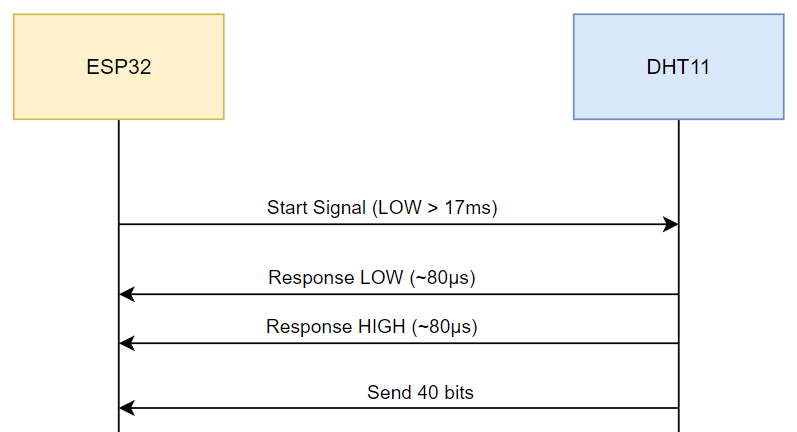
\includegraphics[width=0.7\textwidth]{images/dht-steps.png}
    \caption{Steps in data aquisition from DHT11 sensor}
    \label{fig:dht-steps}
\end{figure}

For the soil moisure data acquisition, I used a resistive soil moisture sensor. The principle of operation is based
on measuring the resistance of the soil. The sensor consists of two probes that are inserted into the soil.
When the soil is dry, the resistance between the probes is high, and when the soil is wet, the resistance is low\cite{s20020363}.
Then an ADC is used to measure the voltage across the probes, which is transofmerd into digital value. In this case, the
ADC is a 12-bit ADC, which means that the digital value can range from 0 to 4095.

The raindrop data is collected using a resistive raindrop sensor. The principle of operation is similar to the soil moisture sensor, but 
in this case, the sensor consists of a plate with two conductive traces that are separated by a small gap.
When the rain falls on the plate, it closes the gap and allows the current to flow between the traces. The 
is connected to an ADC which measures the voltage across the traces.

\begin{figure}[H]
    \centering
    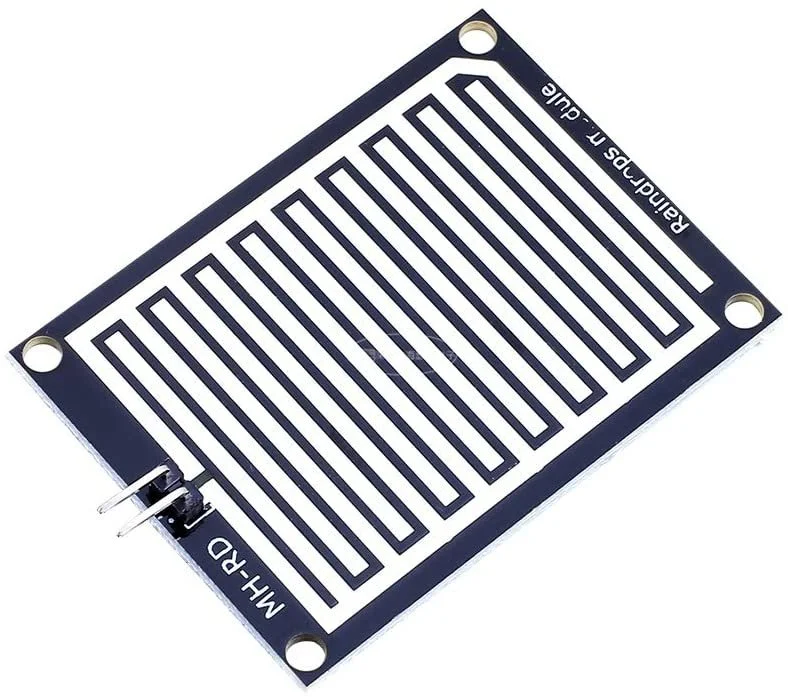
\includegraphics[width=0.4\textwidth]{images/rain-detector-sensor.png}
    \caption{Raindrop sensor based on resistive principle}
    \label{fig:raindrop-sensor}
\end{figure}

Since the water consumption is a very important aspect in agriculture, 
I wanted to add a water flow sensor to the system. For the purpose of this project I used an 
YF-S201 water flow sensor, which is a low-cost sensor that can be used to measure the flow rate of water in a pipe.
The sensor consists of a plastic body with a 
turbine inside that rotates when water flows through it.
The rotation of the turbine generates a pulse signal that can be used to measure the 
flow rate of water.
The sensor has a maximum flow rate of 30 liters per minute and a minimum 
flow rate of 1 liter per minute.
The sensor has three wires: red (VCC), black (GND), and yellow (signal).
At each rotation of the tubine, the sesnsor generates a pulse signal on the signal wire.
This sensor will be used to check if the irrigation system is working properly or not.
The ESP32 counts the number of pulses in a given time interval 
(e.g., 1 second) to calculate the flow rate.
The flow rate can be calculated using the following formula:
\begin{equation}
    \text{Flow Rate} = \frac{\text{Number of Pulses} \times 60}{\text{Time Interval (seconds)}}
\end{equation}
\begin{figure}[H]
    \centering
    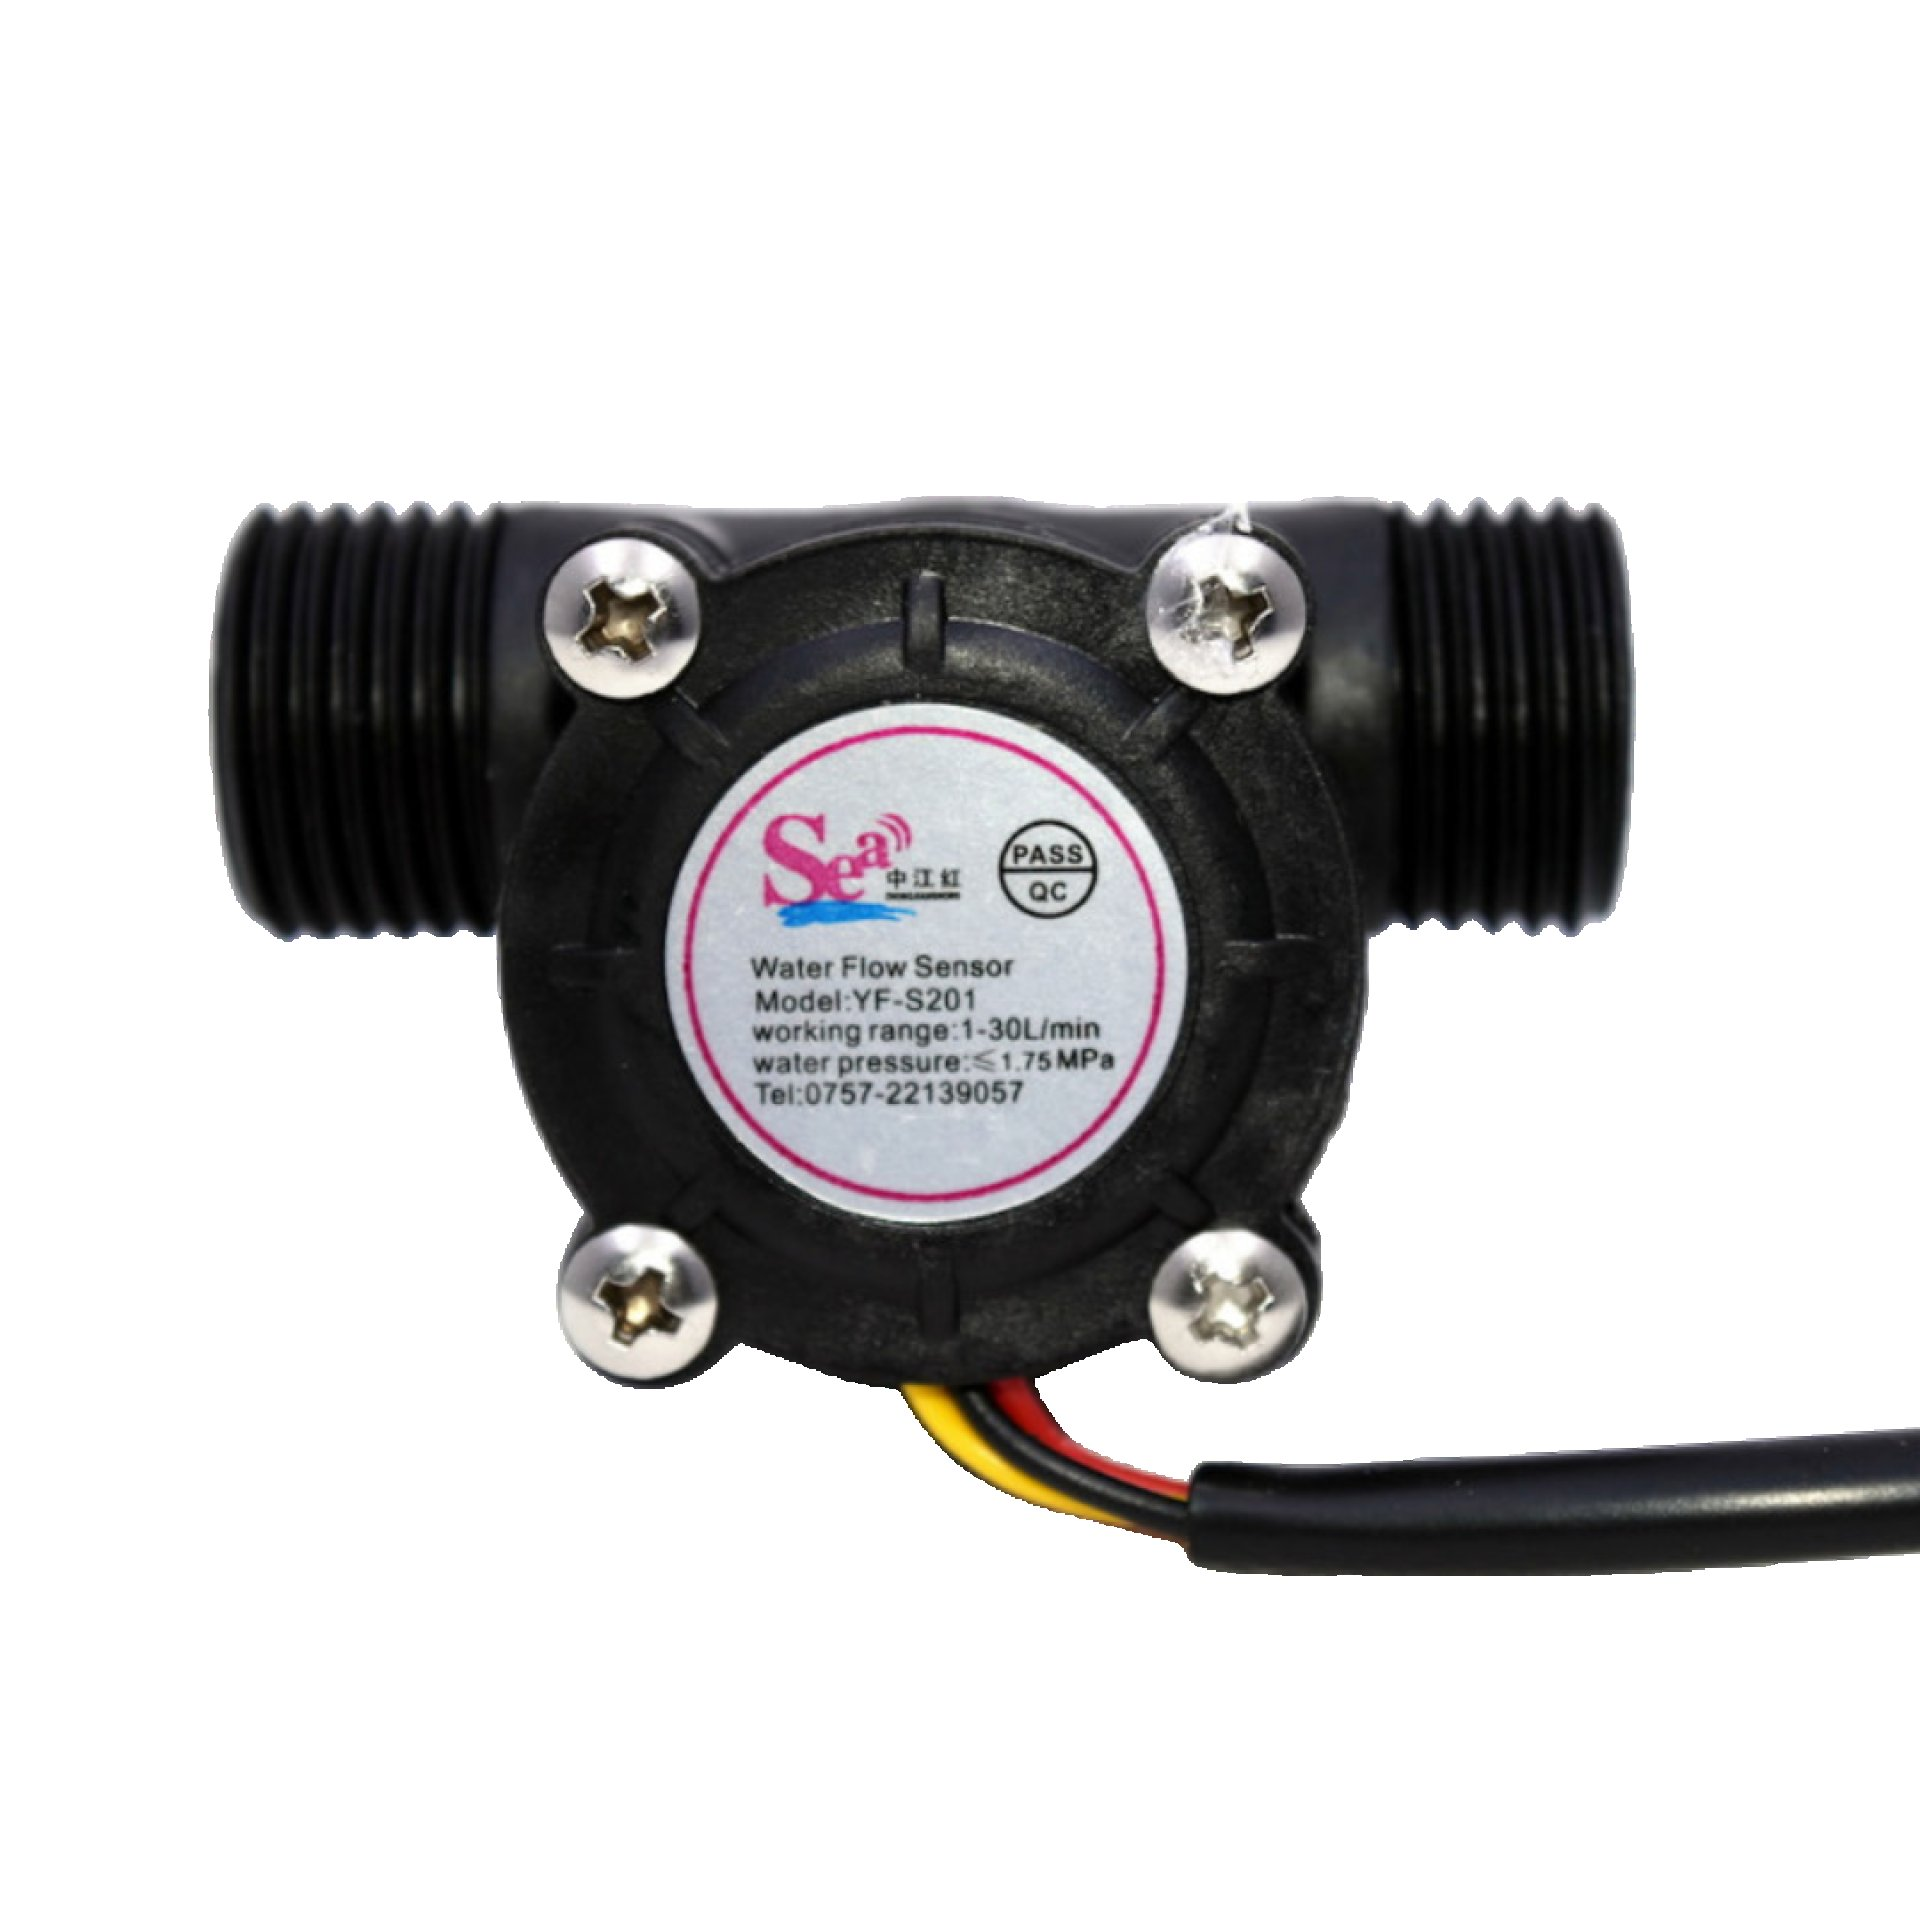
\includegraphics[width=0.5\textwidth]{images/water-flow.jpg}
    \caption{Water flow sensor used in PiIrrigate}
    \label{fig:water-flow-sensor}
\end{figure}

In my implementation the water source is a water tank that will be connected to the irrigation system.
The tank will be equipped with a water temperature sensor. The purpose
of monitoring the water temperature is to ensure that the water is not too cold or too hot for the plants.
The water temperature sensor is a DS18B20 sensor, which is a digital temperature sensor that can be used to measure the temperature of liquids.
The DS18B20 sensor uses the 1-wire digital interface to communicate with the ESP32.
The sensor can measure temperatures from -55°C to +125°C with an accuracy of ±0.5°C.

\begin{figure}[H]
    \centering
    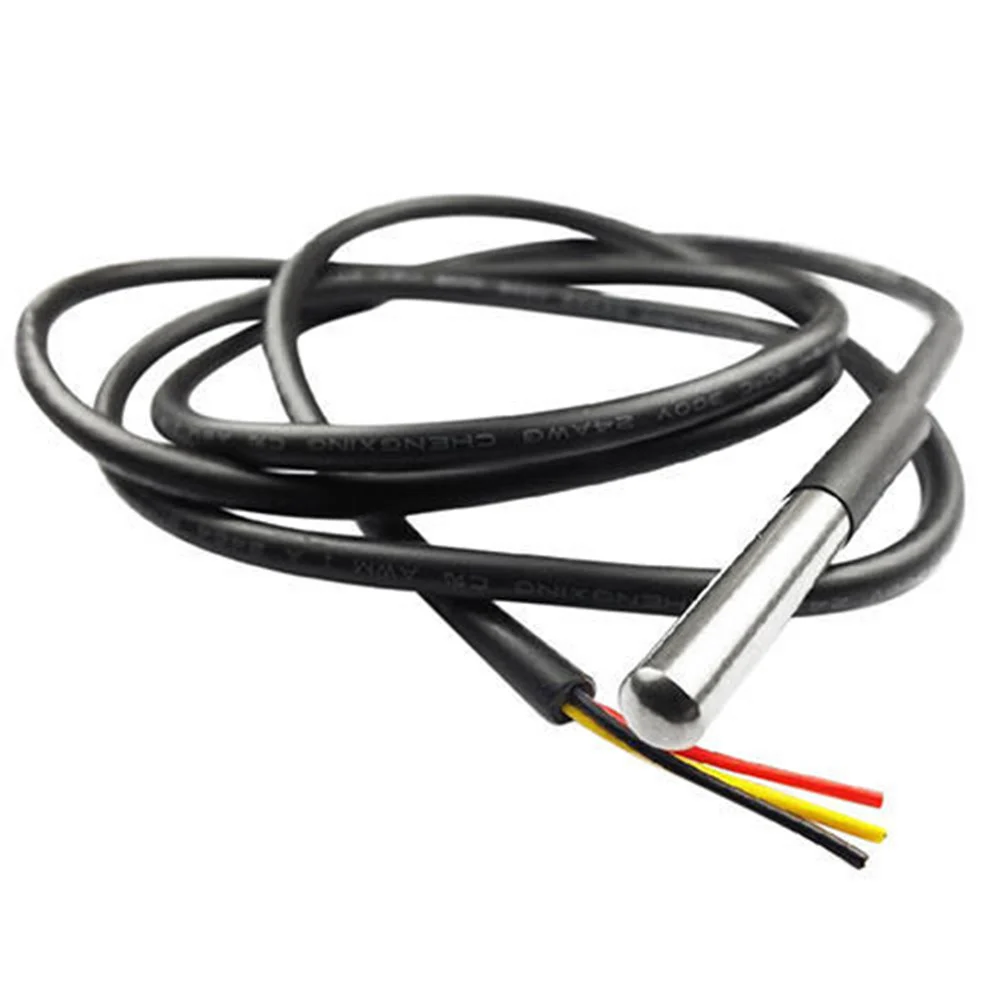
\includegraphics[width=0.5\textwidth]{images/water-temp.png}
    \caption{DS18B20 water temperature sensor used in PiIrrigate}
    \label{fig:ds18b20}
\end{figure}

To be able to locate each node in the field, a GPS module is used. More precisely, I used a NEO-6M GPS module
which is integrated in the LILYGO Meshtastic AXP2101 T-Beam V1.2 ESP32 LoRa development board.

\subsection {Data Transmission}
Once the data is collected from the sensors, it needs to be transmited to the gateway.
The ESP32 nodes use LoRa communication to send the data to the gateway. 
The sensor reading has a period of 10 seconds, which is the default value and it can be changed from the Web Application.
The data collected from the sensors is serialized into a sensor reading structure, 
which is then is included in a LoRa packet structure that will be 
binary serialized and sent over LoRa radio communication.
\begin{lstlisting}[language=C, caption={LoRa packet structure}]
struct LoRaPacket {
    int packetCount;      // Packet count for tracking
    SensorData sensorData; // Sensor data to be sent
    int stationMac[6]; // MAC address of the device
};
\end{lstlisting}

\begin{lstlisting}[language=C, caption={Sensor reading structure}]
struct SensorData {
    time_t timestamp;
    float temperature;
    float humidity;
    float soilMoisture;
    float rainLevel;
    float waterTemp;
    float totalWaterFlow;
    float longitude;
    float latitude;
};
\end{lstlisting}

All the values regarding the environmental data represent the raw
voltages read from the sensors. I chose to sent the raw values, 
because they can be used to calculate any related values in the web api.
This allows a better flexibility in the future.

\section{Raspberry Pi and ESP32 Gateway}
The gateway ESP23 acts like a proxy between the nodes and the Raspberry Pi.
It receives the LoRa packets from the nodes, and then it sends the data to 
the Raspberry Pi using Serial communnication by UART.

UART is an integrated cicuit that plays the most important role in serial communication.
It containts a parallel-to serial converter and a serial-to-parallel converter\cite{uderstandingUart}
\cite{laddha2013review}. The 
parrallel-to-serial converter ia used for data sent from Raspberry Pi to the ESP32,
and the serial-to-parallel converter is used for data sent from the ESP32 to the Raspberry Pi.
The UART frame format is as follows:
\begin{itemize}
    \item Start bit: 1 bit, always 0
    \item Data bits: 5 to 9 bits, usually 8 bits
    \item Parity bit: 1 bit, optional, used for error detection
    \item Stop bit: 1 or 2 bits, always 1
    \item Idle bit: 1 bit, always 1
\end{itemize}

\section {Web Api}
\subsection{Web API}
The web API is developed in \.NET ans it is responsible
for user management, data storage, and communication with the IoT Hub.
It uses Entity Framework Core to interact with the 
PostgreSQL database and SignalR to provide real-time communication.
It uses the controller pattern to handle the HTTP requests. 
I created a controller for each resource in the system,
such as users, zones, data, devices, schedules and cloud to device messages.

\subsubsection{Zone Controller}
Since the first step in the activation process is to verify the code enterede by the
user, I will start describing the zone controller.
Using this controller, the user can create a zone, activate a zone, get the IoT Device connection string, retrieve
all zonees, get a zone by id, and delete a zone. For the database interaction, I created
a zone repository that implements the IZoneRepository interface.
\begin{lstlisting}[caption={Zone Repository interface}]
public interface IZoneRepository
{
    public Task<bool> CreateZone(Zone zone);
    public Task<bool> UpdateZone(Guid Id, string Name, Guid userId);
    public Task<bool> DeleteZone(Guid Id);
    public Task<Zone> GetZoneById(Guid Id);
    public Task<Zone> GetZoneByName(string name);
    public Task<IEnumerable<Zone>> GetAllByUserId(Guid Id);
}
\end{lstlisting}

The controller is also using the IoTDeviceManager service to manage the
IoT devices in Azure IoT Hub, which implement the IioTDeviceManager interface and 
is repsonsible for creating, deleting, and checking the existence of IoT devices.

\begin{lstlisting}[caption={IoT Device manager interface}]
public interface IiotDeviceManager
{
    public Task<bool> CreateIotDevice(string zoneId);
    public Task<string> GetDeviceConnectionString(string zoneId);
    public Task<bool> DeviceExists(string zoneId);
    public Task<bool> DeleteIotDevice(string zoneId);
}
\end{lstlisting}

\subsection{Zone Activation}
The Raspbery Pi represents a "zone" in the system and it connects to a single Azure IoT Hub Device. Each zone needs to
connect to the Azure IoT Hub Device using a connection string. To obtain that connection string, a a reuest is sent 
to the web API to create a new zone. The web api will create the zone in the database and it will create a new IoT Device
in the Azure IoT Hub. The connection string will be returened to the "zone". Aftr that, the RaspberryPi won't send any 
reading to the cloud, the sending of the data will be done only when the zone is activated.
The activation process is as follows:
\begin{enumerate}
    \item The user enters the code displayed on the Raspberry Pi OLED display in the web application.
    \item The web application sends the code to the web API.
    \item The web API verifies the code and activates the irrigation zone.
    \item The web API sends a message to the Iot Device to activate the irrigation zone.
    \item The Raspberry Pi receives the message from Azure IoT Hub and activates the irrigation zone.
    \item The Raspberry Pi sends a message to the ESP32 nodes to start collecting data from the sensors.
\end{enumerate}

\begin{figure}[H]
    \centering
    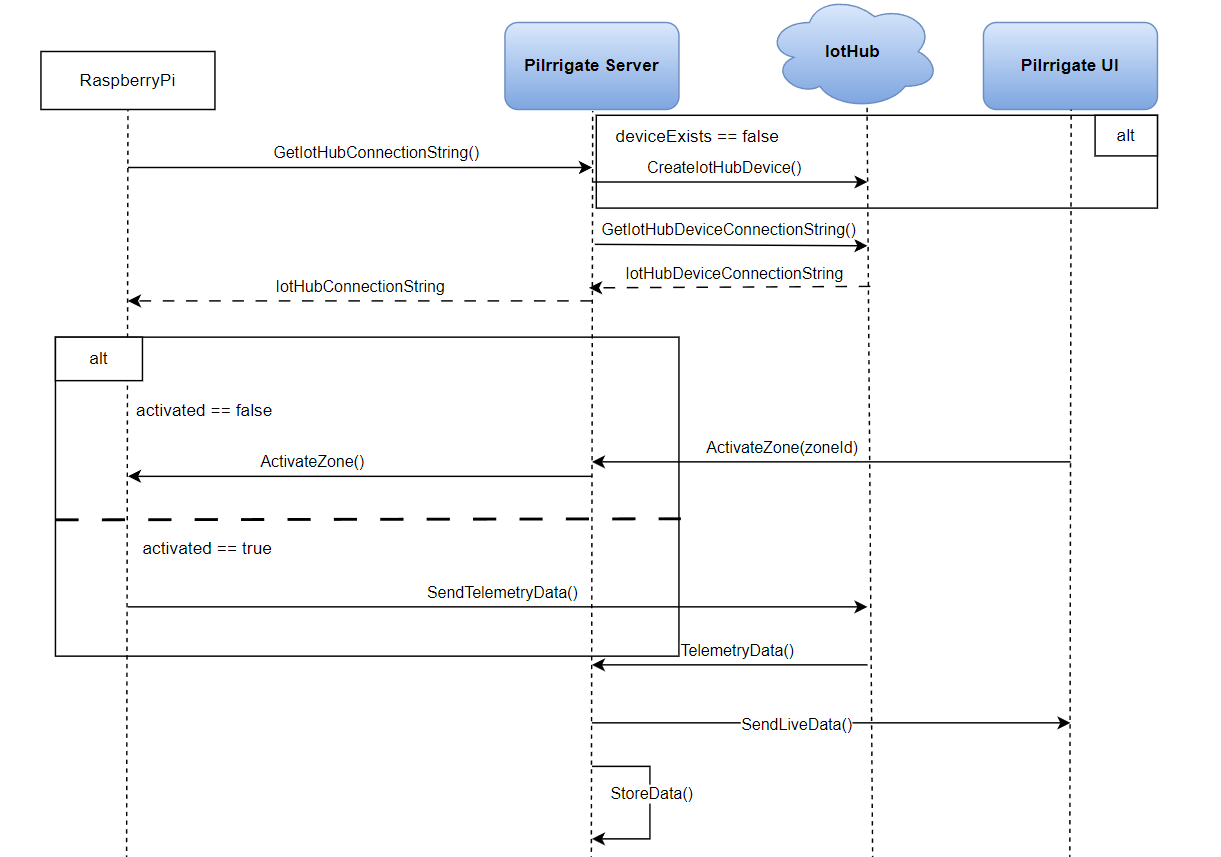
\includegraphics[width=0.9\textwidth]{images/activation.png}
    \caption{Zone activation process}
    \label{fig:zone-activation}
\end{figure}

\subsubsection{Data Controller}
The data controller is used to retrieve stored data from the Web API. This data is stored in the PostgreSQL database and
it will be used to display historical data and analytics in the web application.
It provides endpoints for:
\begin{itemize}
    \item Get all data for a zone, including the data for all devices in that zone.
    \item Get data for a certain period of time.
    \item Get all data foor a device.
    \item Get data for a device for a certain period of time.
\end{itemize}

IData repository is used to interact with the database and it implments the IDataRepository interface.
\begin{lstlisting}
public interface IDataRepository
{
    public Task StoreData(SensorReading sensorReading);
    public Task<IEnumerable<SensorReading>> GetTimedZoneData(DateTime from, DateTime to, Guid zoneId);
    public Task<IEnumerable<SensorReading>> GetTimedDeviceData(DateTime from, DateTime to, Guid zoneId, string deviceId);
    public Task<IEnumerable<SensorReading>> GetAllZoneData(Guid zoneId);
    public Task<IEnumerable<SensorReading>> GetAllDeviceData(Guid zoneId, string DeviceId);
}
\end{lstlisting}
\subsubsection{Device Controller}
The device controller is used to manage the devices in the system.
It provides endpoints for:
\begin{itemize}
    \item Get all devices for a zone.
    \item Get all devices for a user.
    \item Get a device by id.
    \item Get a device by MAC address.
    \item Register a new device.
\end{itemize}

\subsubsection{C2D Controller}
The C2D (Cloud to Device) controller is used to manage the cloud to device messages in the system.
It provides only one endpoint to send a message to a device. The endpoint accepts a C2DMesageRequest object, 
which contains the zoneId, and an object of type C2DMethodCall, which contains the the deviceId, the method name, and a list of parameters.
\begin{figure}[H]
    \centering
    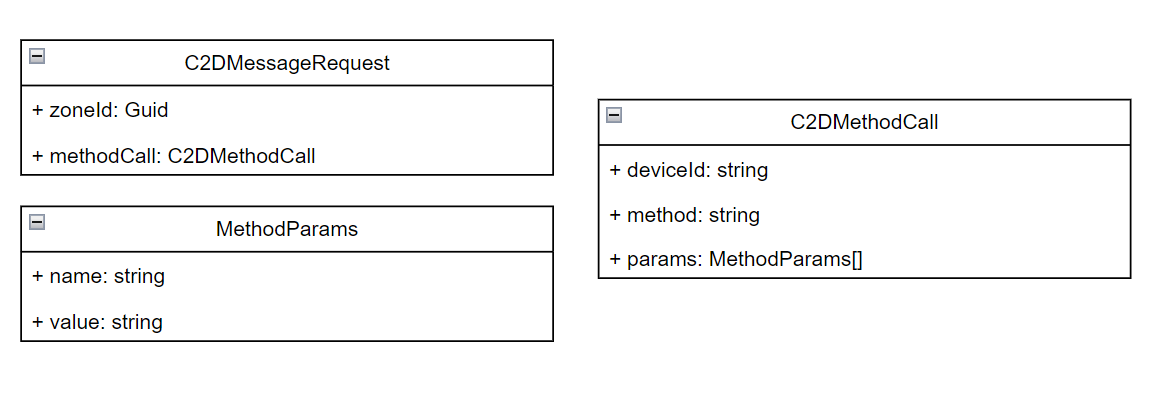
\includegraphics[width=0.8\textwidth]{images/c2d-message-request.png}
    \caption{C2D Message Request object}
    \label{fig:c2d-request}
\end{figure}

\subsubsection{Schedule Controller}
The schedule controller is used to manage the irrigation schedules in the system.
It provides endpoints for:
\begin{itemize}
    \item Get all schedules.
    \item Get a schedule by id.
    \item Create a new schedule.
    \item Update an existing schedule.
    \item Delete a schedule.
\end{itemize}

The Schedule object is defined as follows:
\begin{figure}[H]
    \centering
    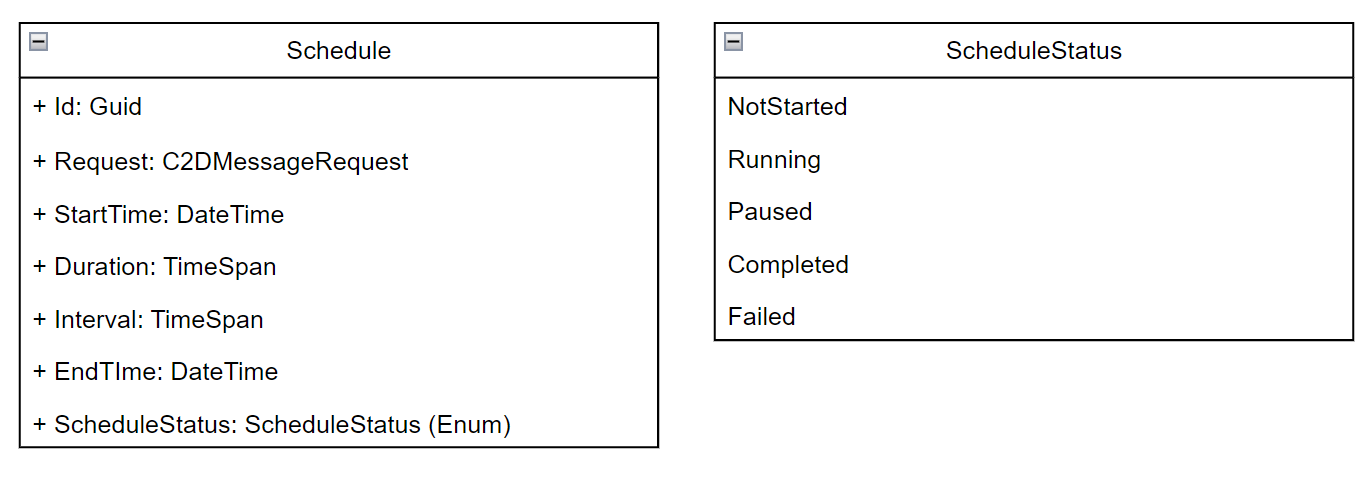
\includegraphics[width=0.8\textwidth]{images/schedule.png}
    \caption{Schedule object}
    \label{fig:schedule-object}
\end{figure}

\begin{enumerate}
    \item The Id is a unique identifier for the schedule.
    \item The Request is an object of type C2DMesageRequest that contains the zoneId, deviceId, method name, and parameters.
    \item The StartTime is the time when the schedule should start.
    \item The EndTime is the time when the schedule should end.
    \item The Interval is the time interval between two consecutive executions of the schedule.
    \item The Duration is the duration of the schedule execution.
    \item The ScheduleStatus is the status of the schedule, which can be NotStarted, Running, Paused, Completed, Failed.
\end{enumerate}

The user can create a new schedule using the UI of the web application,
which will send a request to the web API to create a new schedule. 
The web API will validate the request and create a new schedule in the database.
A bragraound service will be used to check and execute the schedules. The background service will run 
every minute and check if there are any schedules that should be executed or stoped. To be more robust, the duration 
of the schedule, as well as the start and end time, will be sent to the Raspberry Pi, wich will also check if 
the schedule should be executed or stopped. This way if the Web API or the network connectivity is down, 
the Raspberry Pi will still be able to execute the schedules.

A background service is used to check the schedules. A baground services is a service that implements
the IHostedService interface and runs tasks in the background. It is used to perform long-running tasks and
it implements the StartAsync and StopAsync methods \cite{IHostedService}.


\subsubsection{User Controller}
As the user needs to be authenticated to access the web API,
I created a user controller that handles user registration and login.

For accessing the user data, UserRepository is used, which implements the IUserRepository interface.
The authorization is done using JWT tokens, 
which are generated when the user logs in. To handle all the logic related to 
JWT tokens, I created a JWT service that implements the IJwtService interface.
Besides IUserRespository, and IJwtService, the UserService is also using
IPasswordHasher to hash the user passwords. This provides abstraction
for hashing and verifying passwords, 
allowing for easy integration with different hashing algorithms. For the moment,
the implementation uses SHA256 hashing algorithm, 
but it can be easily changed to any other algorithm. In the future, I plan to replace
this with Microsoft.AspNetCore.Identity, 
which provides a more secure and flexible way to handle user 
authentication and authorization and it is widely used in the \.NET community.

\begin{lstlisting}[caption={User Repository interface}]
public interface IUserRepository
{
    Task<User> GetByIdAsync(Guid id);
    Task<User> GetByEmailAsync(string email);
    Task<IEnumerable<User>> GetAllAsync();
    Task<bool> CreateAsync(User user);
    Task<bool> UpdateAsync(User user);
    Task<bool> DeleteAsync(Guid id);
}
\end{lstlisting}

\begin{lstlisting}[caption={JWT Service interface}]
public interface IJwtService
{
    string GenerateJwtToken(User user);
    bool ValidateToken(string token);
}
\end{lstlisting}

\begin{lstlisting}[caption={Password Hasher interface}]
public interface IPasswordHasher
{
    string HashPassword(User user, string password);
    bool VerifyPassword(User user,string hashedPassword, string providedPassword);
}
\end{lstlisting}

\subsubsection{Registration Flow}
The registration flow is as follows:
\begin{enumerate}
    \item The user fills the registration form in the web application.
    \item The web application sends the request to the web API. More sdpecifically, 
    it sends a POST request to the register endpoint of the user controller. The controller
    receives the request as an object of type RegisterRequest.
    \item The request is being validated by the web API.
    \item If the request is valid, the web API creates a new user in the database
    \item The web API generates a JWT token and it sends back an object of type AuthResult.
    \item The web application receives the AuthResult object and stores the JWT token in the local storage.
\end{enumerate}

The registration flow is shown in the figure below.
\begin{figure}[H]
    \centering
    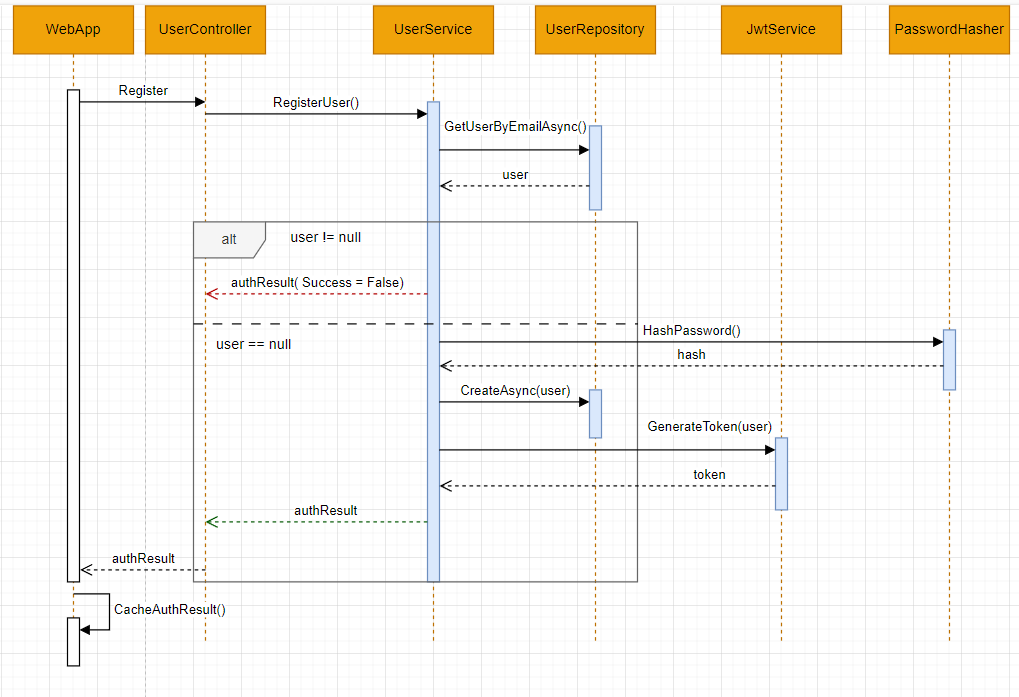
\includegraphics[width=0.9\textwidth]{images/registration-flow.png}
    \caption{Registration flow}
    \label{fig:registration-flow}
\end{figure}

The AuthResult object and the RegisterRequest object are defined as follows:
\begin{figure}[H]
    \centering
    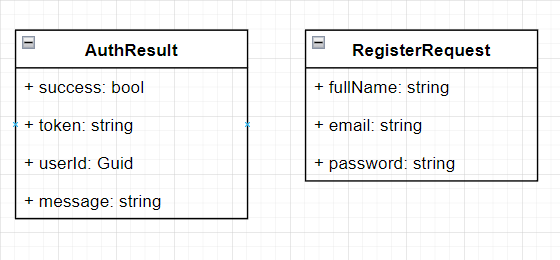
\includegraphics[width=0.8\textwidth]{images/auth-request.png}
    \caption{AuthResult and RegisterRequest objects}
    \label{fig:auth-result}
\end{figure}

\subsubsection{Login Flow}
The login flow is similar to the registration flow, but it does not create a new user.
The login flow is as follows:
\begin{enumerate}
    \item The user fills the login form in the web application.
    \item The web application sends a POST request to the login endpoint of the user controller. The controller
    receives the request as an object of type LoginRequest.
    \item The request is being validated by the web API.
    \item If the request is valid, the web API checks if the user exists in the database.
    \item If the user exists, the web API verifies the password and generates a JWT token.
    \item The web API sends back an object of type AuthResult.
    \item The web application receives the AuthResult object and stores the JWT token in the local storage.
\end{enumerate}

The login flow is shown in the figure below.
\begin{figure}[H]
    \centering
    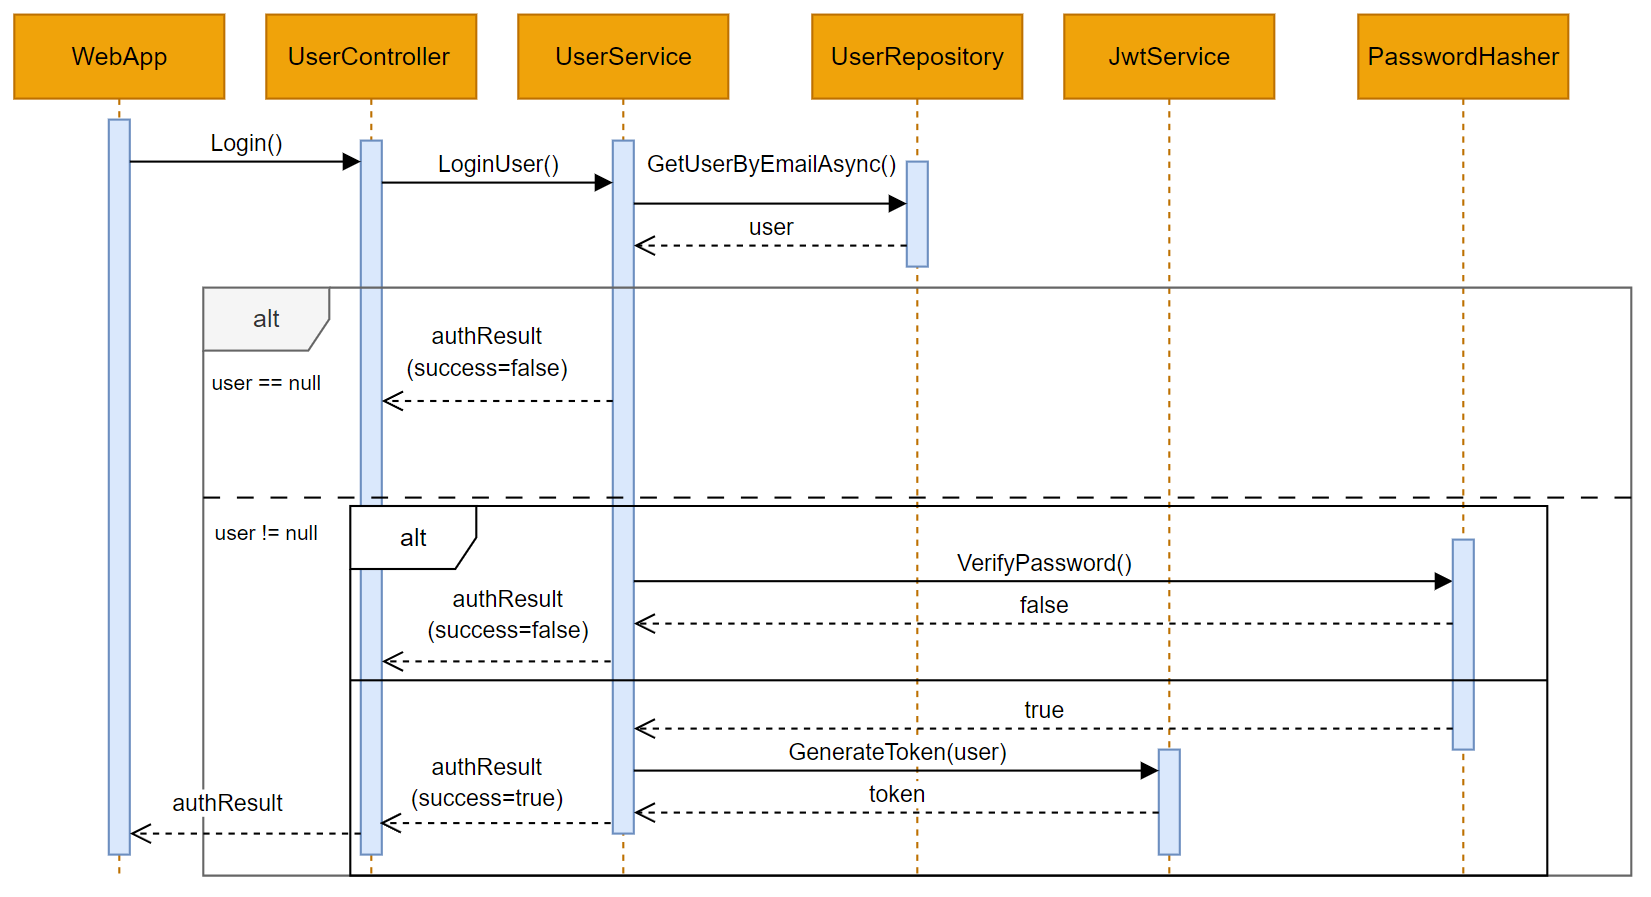
\includegraphics[width=0.9\textwidth]{images/login-flow.png}
    \caption{Login flow}
    \label{fig:login-flow}
\end{figure}

\section {Web Application}
The frontend interface of the smart irrigation system was implemented using Angular. The web application serves as the main
point of interaction between the user and the backend system. It allow the users to monitor the environmental conditions
in real-time and manually controll irrigation events.

The communication between the frontend and web API is done via 2 methods: HTTP requests - for fetching sensor data, trigger
irrigaiton actions and display system status and SignalR - for sending live data from the API to fronend. In the HTTP requests,
a JWT token is included, ensuring secure access to system's features.

The user interface is divided into several key components: Dasboard, Devicem Management, Configuration, Schedules, Data Analytics and Live Charts.
The user can navigate between these components using a side drawer menu that is visible in \ref{fig:dashboard-page}. 
Each value is displayed in a separate gauge-style widget to improve the readability.In this section the user can also controll the irrigation system.
Now I will describe each component in detail, starting with the landing page.

\subsection{Landing Page}
The landing page is the first page that the users sees when they access the web application.
It presints the user with a brief introduction into the system and it provides the the user with the main 
features of the system. The page is responsive, meaning that it can be accessed from any device,
including mobile phones and tablets. The page contains a scrollable
carousel with the main features of the system and a call to action button that redirects the user to the registration page.
In the following figure you can see the landing page on a desktop and on a mobile phone. 
\begin{figure}[H]
    \centering
    \begin{minipage}{0.5\textwidth}
        \centering
        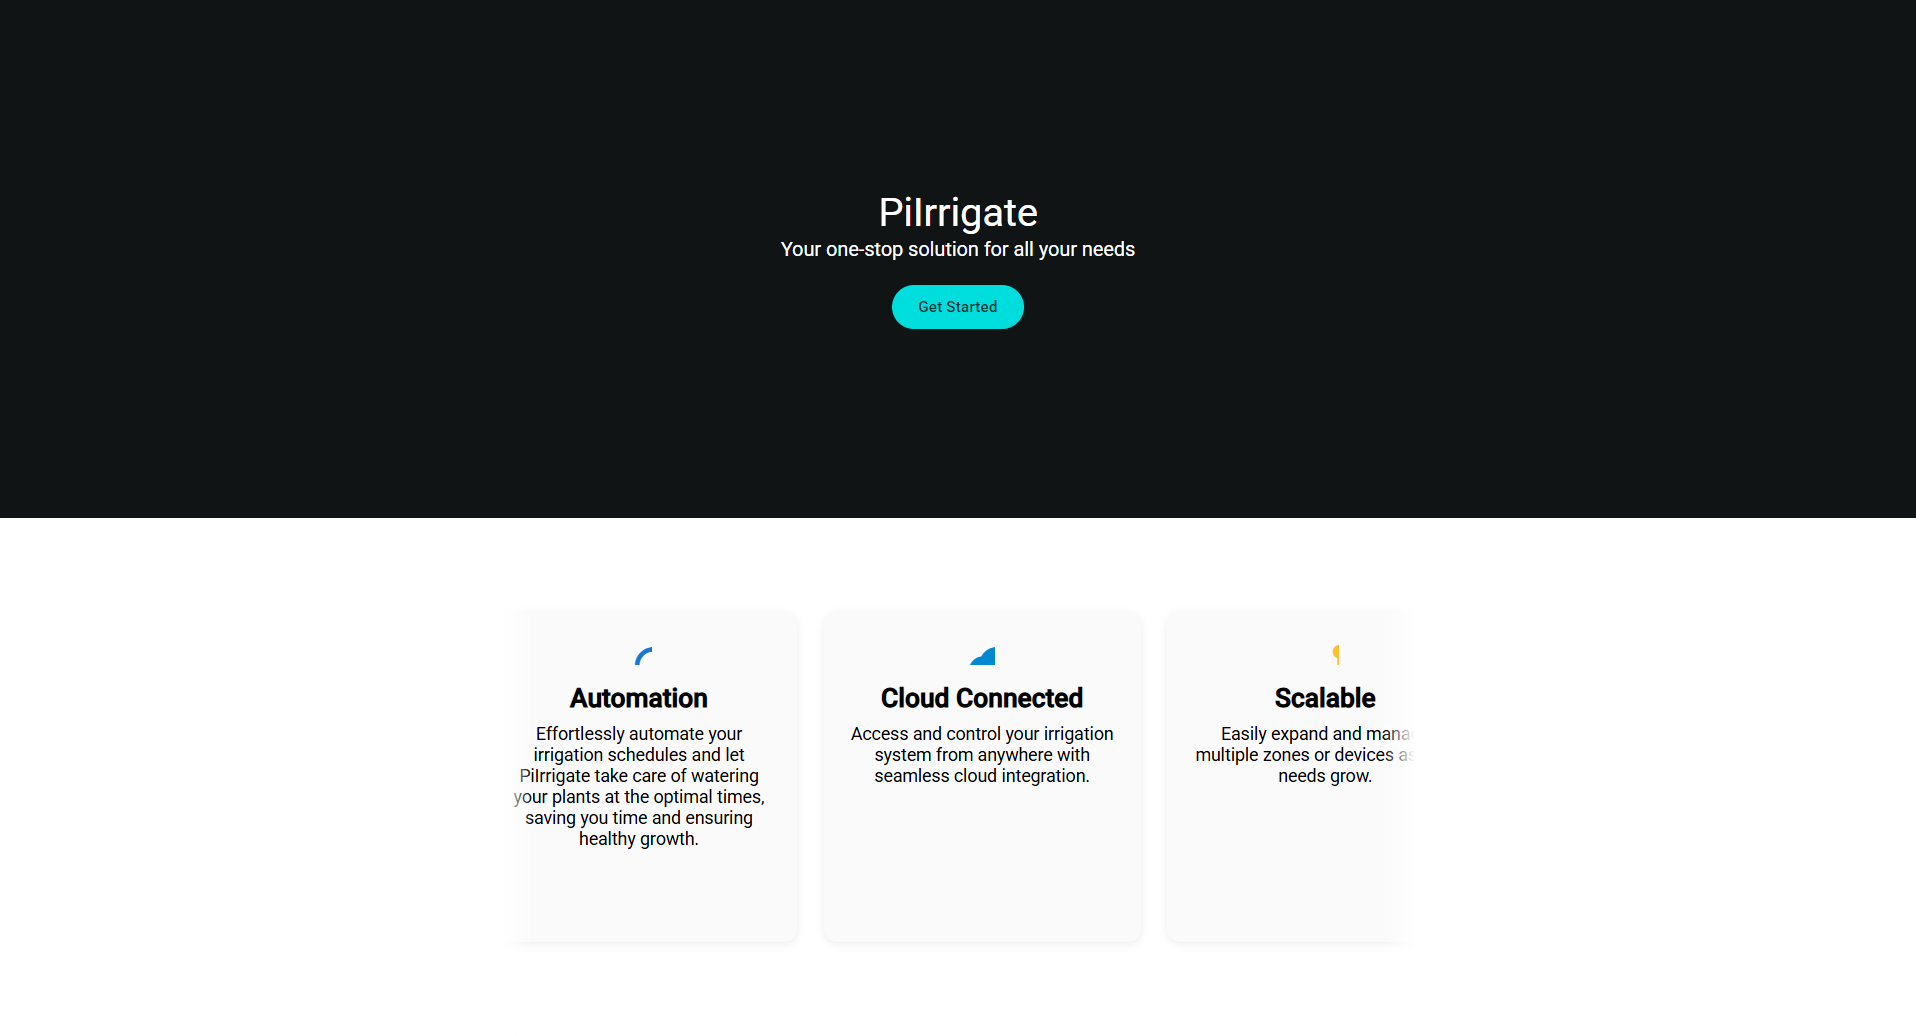
\includegraphics[width=\textwidth]{images/landing_page.png}
        \label{fig:landing-page-desktop}
    \end{minipage}\hfill
    \begin{minipage}{0.3\textwidth}
        \centering
        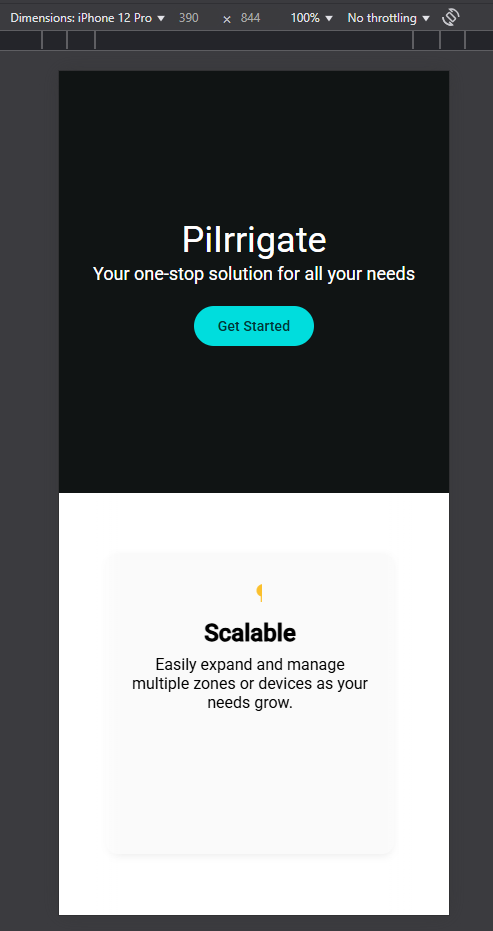
\includegraphics[width=\textwidth]{images/landing_12_pro.png}
        \label{fig:landing-page-mobile}
    \end{minipage}
    \caption{Landing page of the web application}
\end{figure}

\subsection{Register and Login}
The registration and the Login pages are designed to be as simple as possible. 
Registration page contains a form with the following fields: Full Name, Email, Password,
, Confirm Password and a checkbox for accepting the terms and conditions. 
The login page contains a form with only 2 fields: Email and Password.


\begin{figure}[H]
   \centering
    \begin{minipage}{0.3\textwidth}
        \centering
        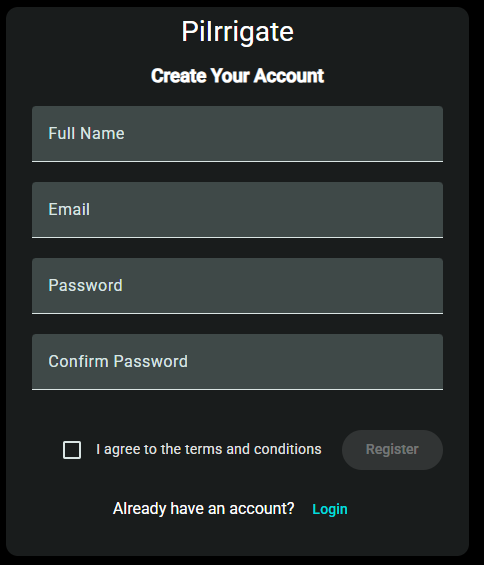
\includegraphics[width=\textwidth]{images/register_page.png}
        \label{fig:register-page}
    \end{minipage}\hfill
    \begin{minipage}{0.3\textwidth}
        \centering
        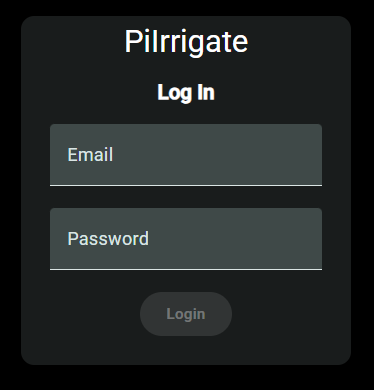
\includegraphics[width=\textwidth]{images/login.png}
        \label{fig:login-page}
    \end{minipage}
    \caption{Register and Login pages}
\end{figure}

Now I will describe the registration and login flows. Afther ther user presses the
call to action button from the landing page, he is redirected to the registraiton page. 
If the users fills the registration form and presses the register button it will be automatically
logged in and redirected to the Dashboard. From the register page he can navigate to the login page where
he can login. If the login fails, the user will can reset his password and try again.
Bellow is presented the user flow diagram.
\begin{figure}[H]
    \centering
    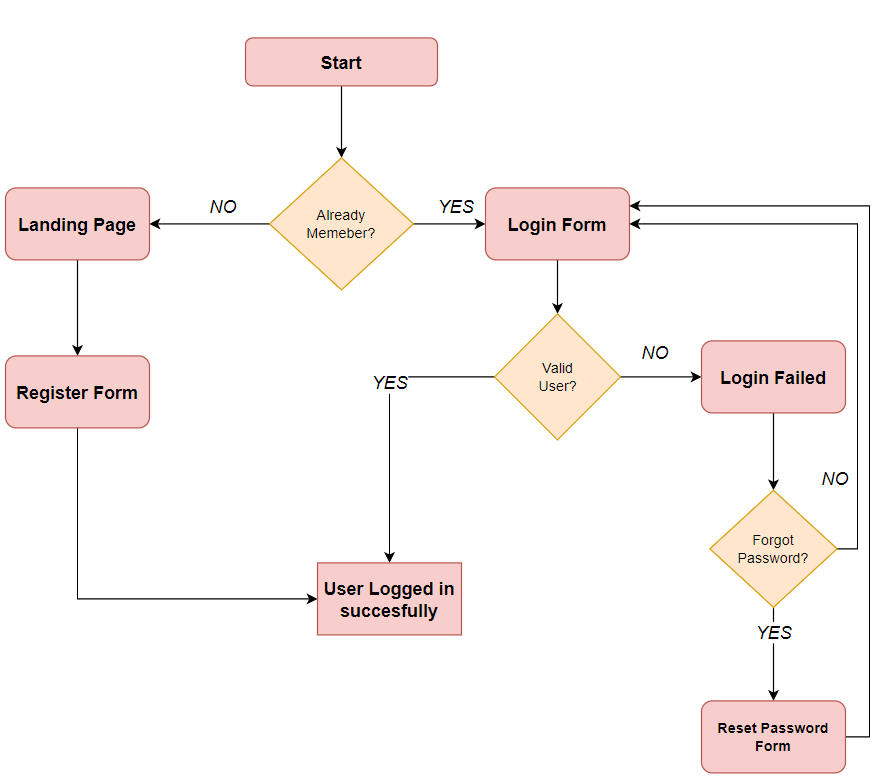
\includegraphics[width=0.5\textwidth]{images/user_flow.png}
    \caption{User flow}
    \label{fig:user-flow}
\end{figure}

\subsection{Dashboard}
The Dashboard components contains several widgets some widgets are used to display live data
and others are used to controll the irrigation system. 
The live data widgets are: Live Soil Moisture, Live Temperature, Live Humidity,
Live Water Flow Rate and Live Water Temperature. In the control widget, the user can
start or stop the irrigation process.

\begin{figure}[H]
    \centering
    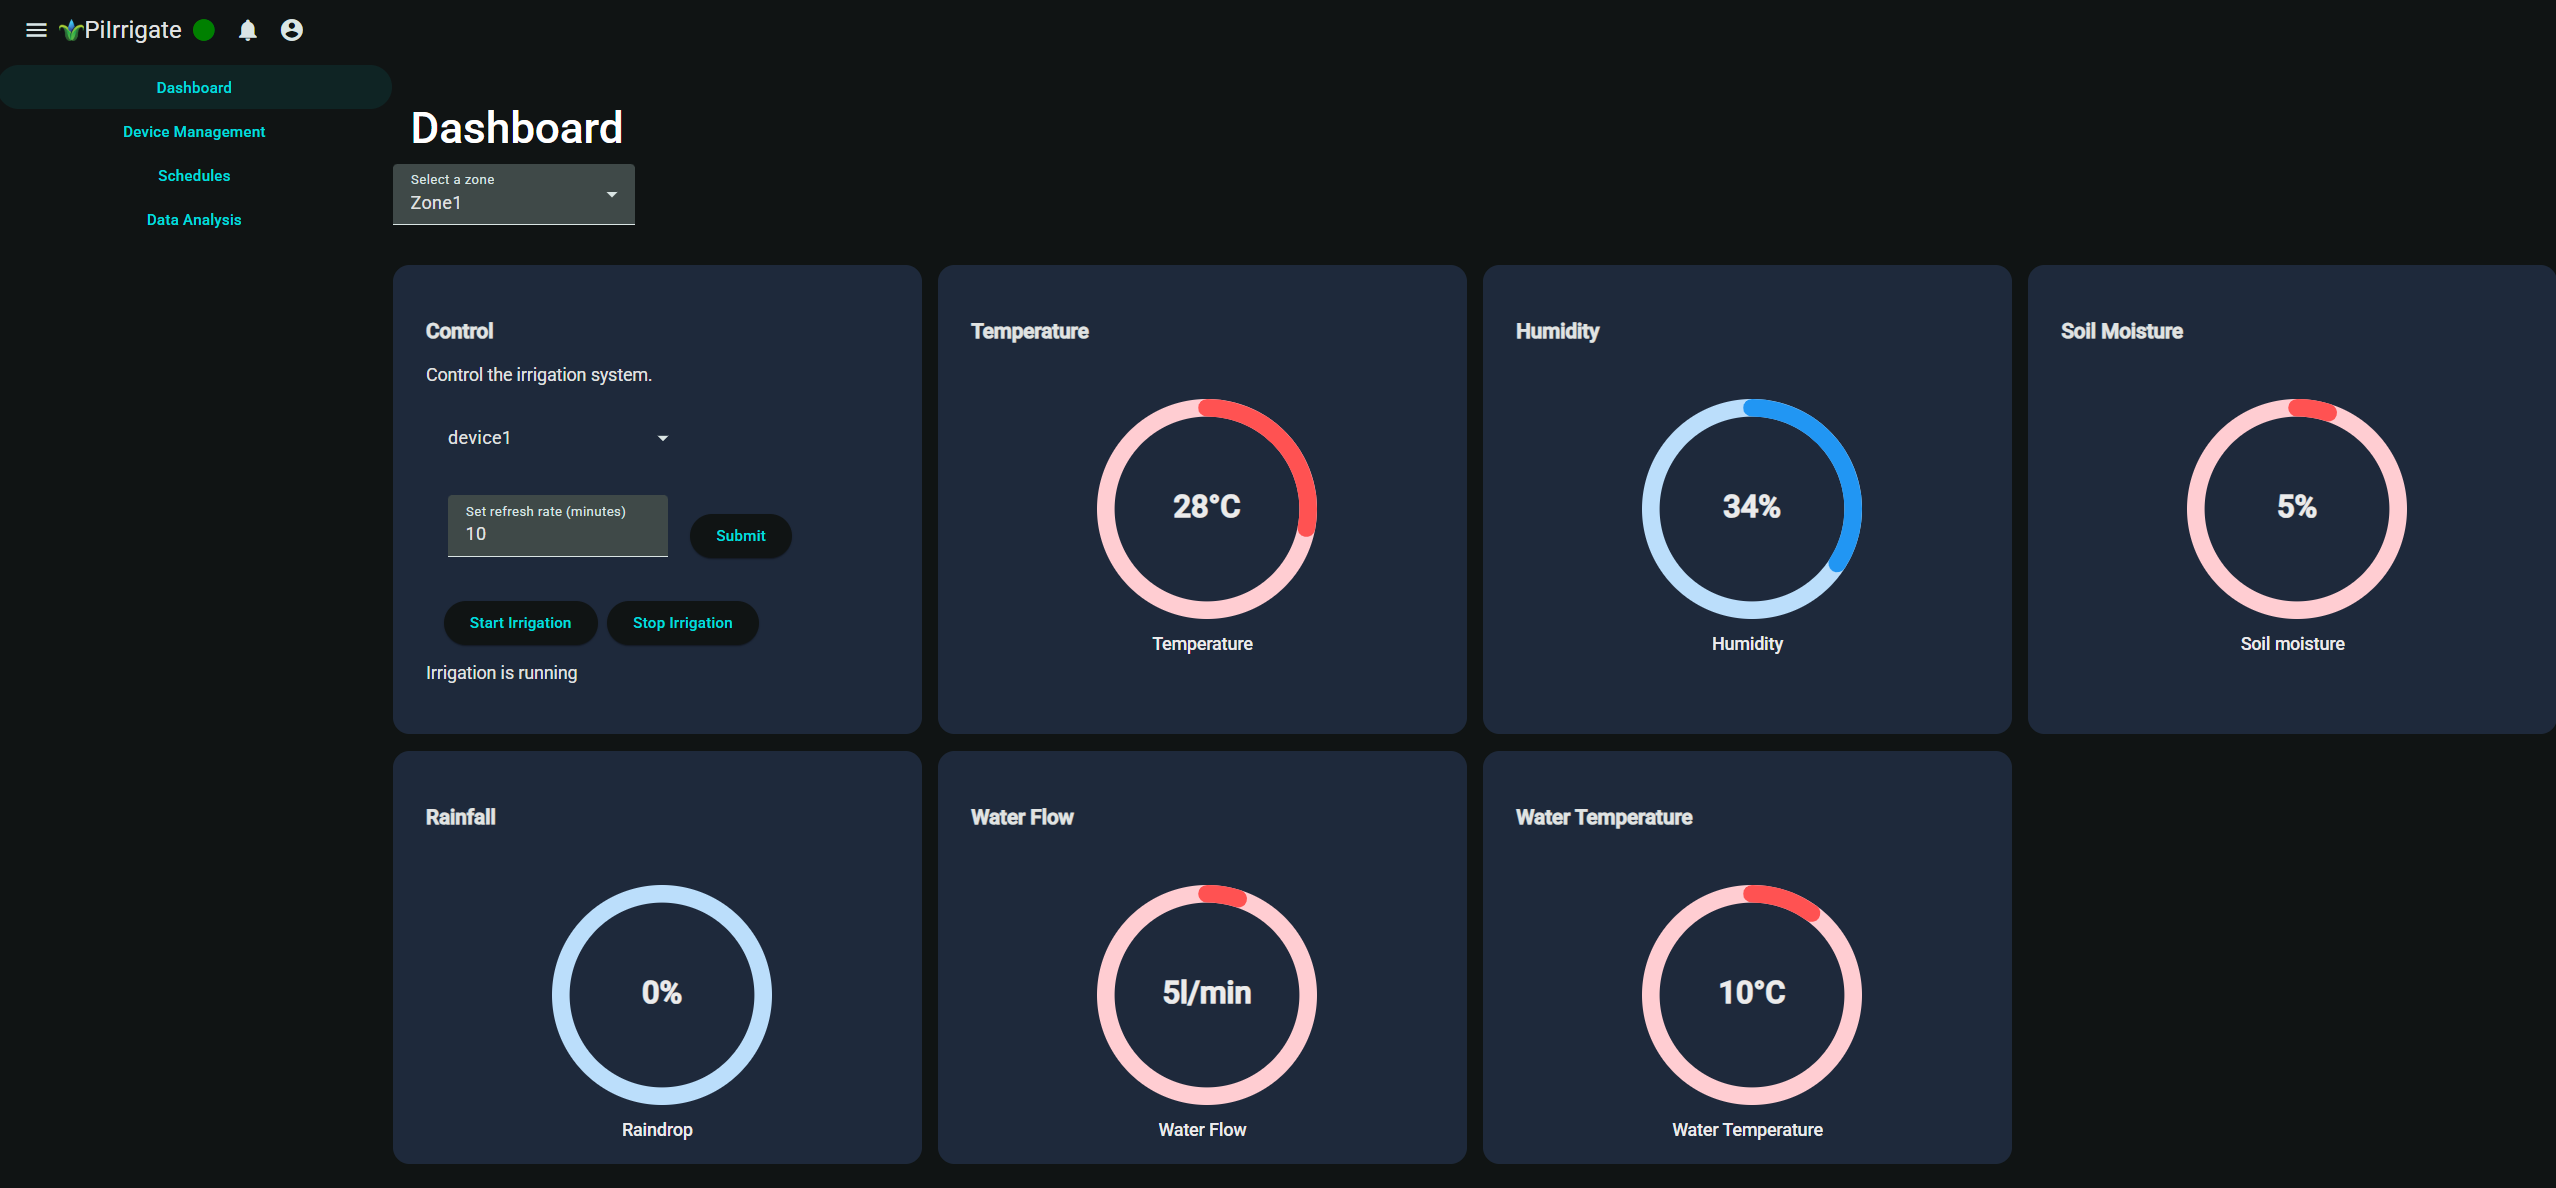
\includegraphics[width=0.8\textwidth]{images/dashboard.png}
    \caption{Dashboard page}
    \label{fig:dashboard-page}
\end{figure}

% TO DO add more details about UI
\subsection{Device Management}
In this section the user canm visualize all the devices that are registered in the system.
The devices are display in tree format, where each zone is a parent node and the devices are the child nodes.
Two buttons are available in this section: one for registering a new device and another for registering a new zone.
Also, the user can delete a device or a zone by clicking the button from the right side of the tree. See \ref{fig:device-management} 
for the Device Management page.
\begin{figure}[H]
    \centering
    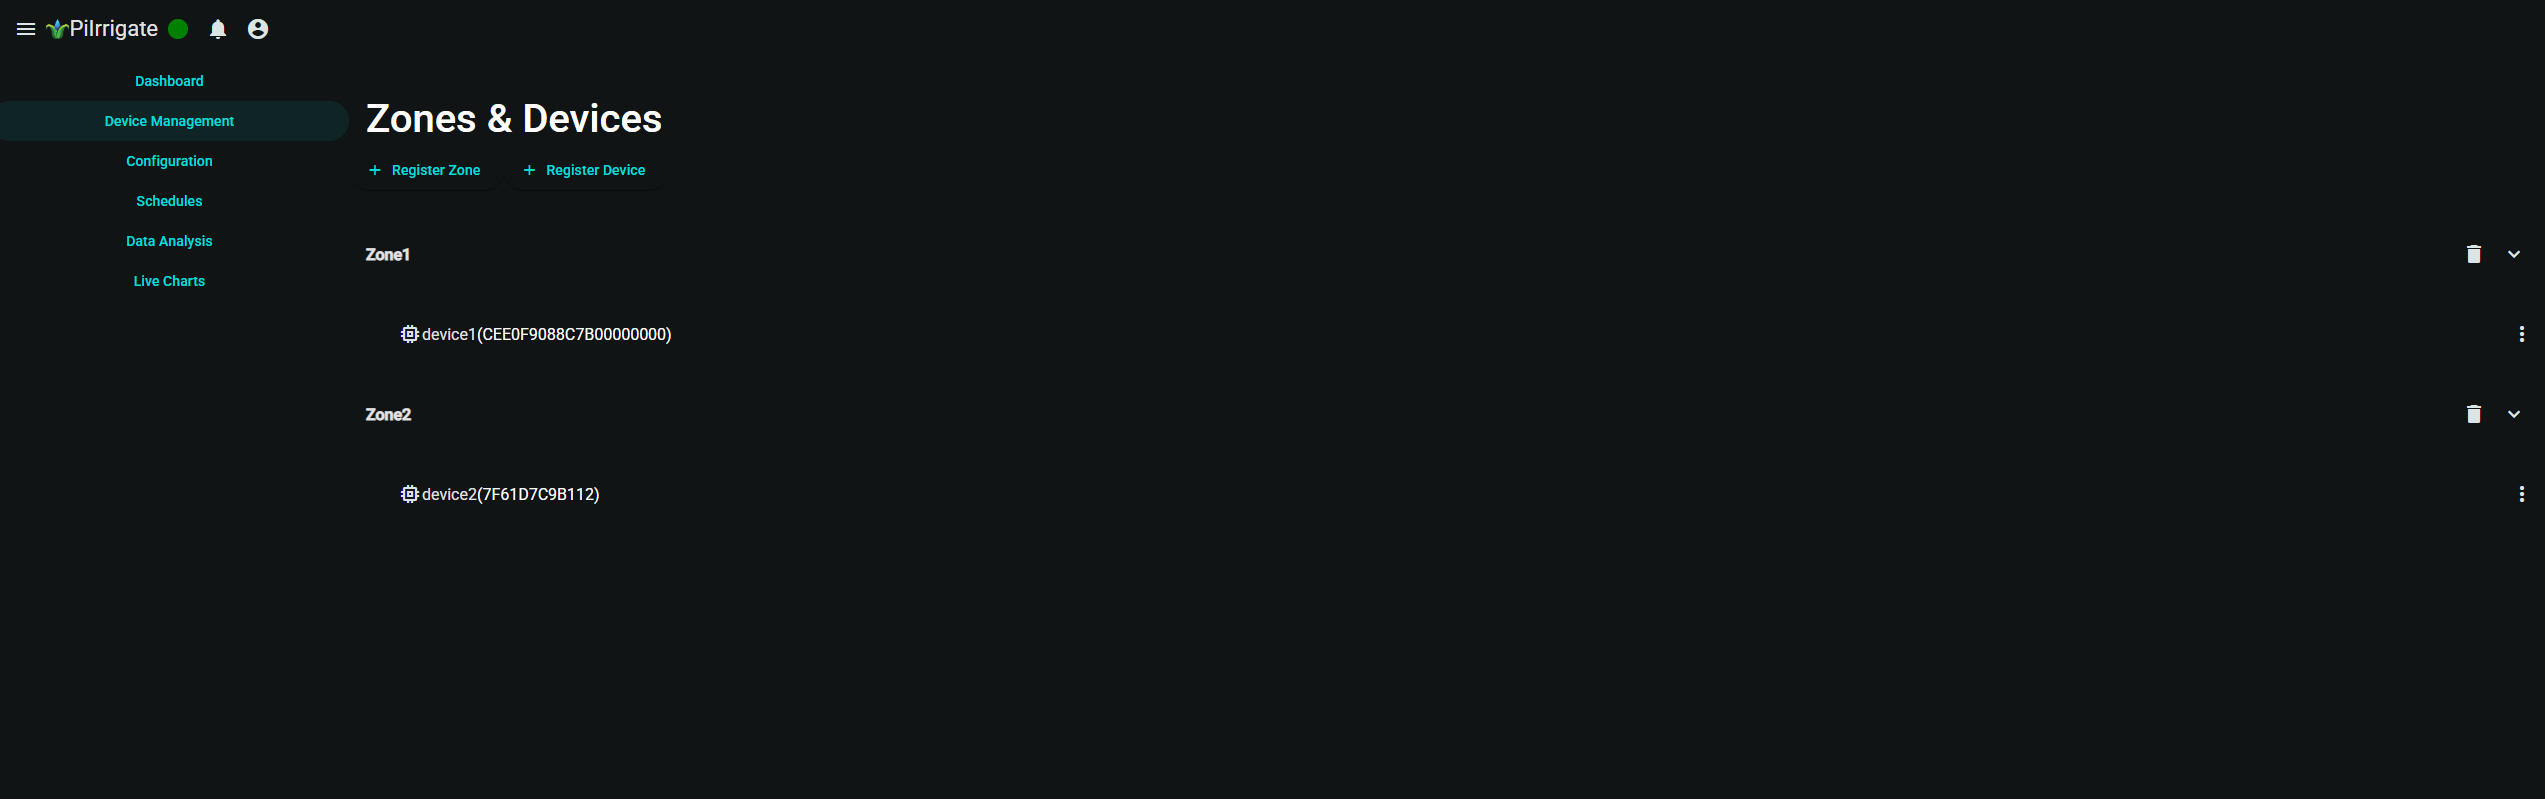
\includegraphics[width=0.8\textwidth]{images/device_management.png}
    \caption{Device Management page}
    \label{fig:device-management}
\end{figure}

\subsection {Configuration}
In the configuration section the user can configure the system settings. The user can change the following settings:
soil moisture threshold, water flow rate threshold, water temperature threshold, raindrop sensor threshold, the 
period of the sensor readings, and to enable or disable notifications or automation. A reset button will be added in the future. See 
\ref{fig:configuration-page} for the configuration page.

\begin{figure}[H]
    \centering
    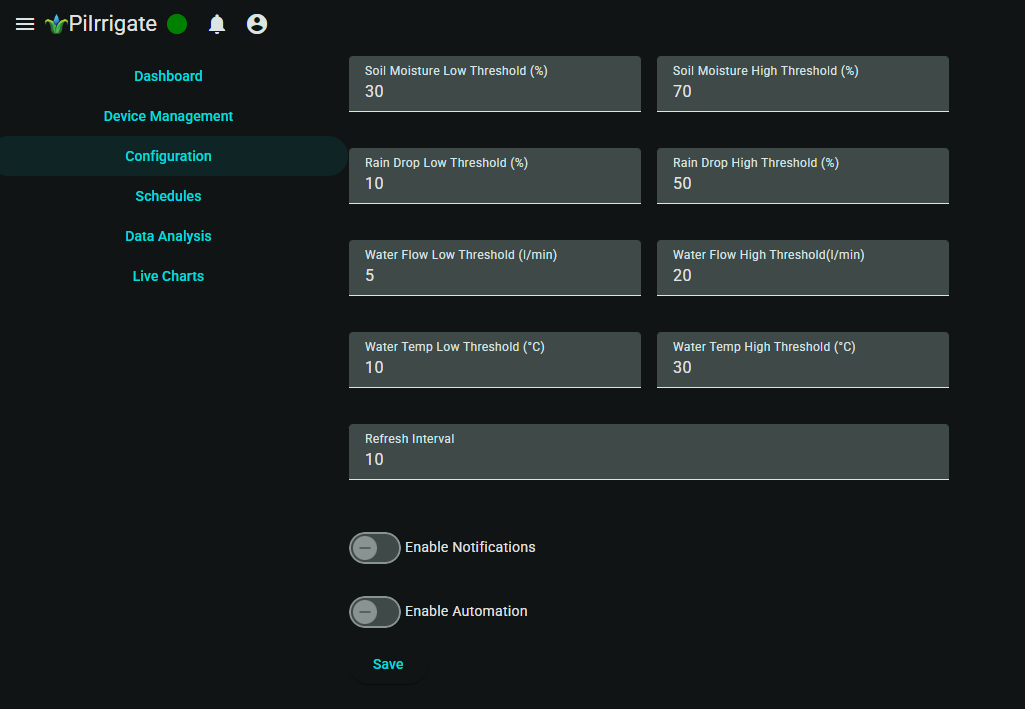
\includegraphics[width=0.8\textwidth]{images/configuration.png}
    \caption{Configuration page}
    \label{fig:configuration-page}
\end{figure}

\subsection{Schedules}
In this section the user can view, create, update and delete irrigation schedules. When the "Create Schedule" button is pressed, a dialog
will open wehre the user can fill the schedule details. THe dialog contains a form with the following fields:
Zone, Device, Start Time, End Time, Interval and Duration. For the Start and End Time fileds, a date range picker is used,
which allows the user to select a date range for the schedule. The interval is the time interval between two consecutive executions of the schedule in hours.
The duration is the duration of the schedule execution in minutes. See \ref{fig:schedules-page} for the Schedules page. 

\begin{figure}[H]
    \centering
    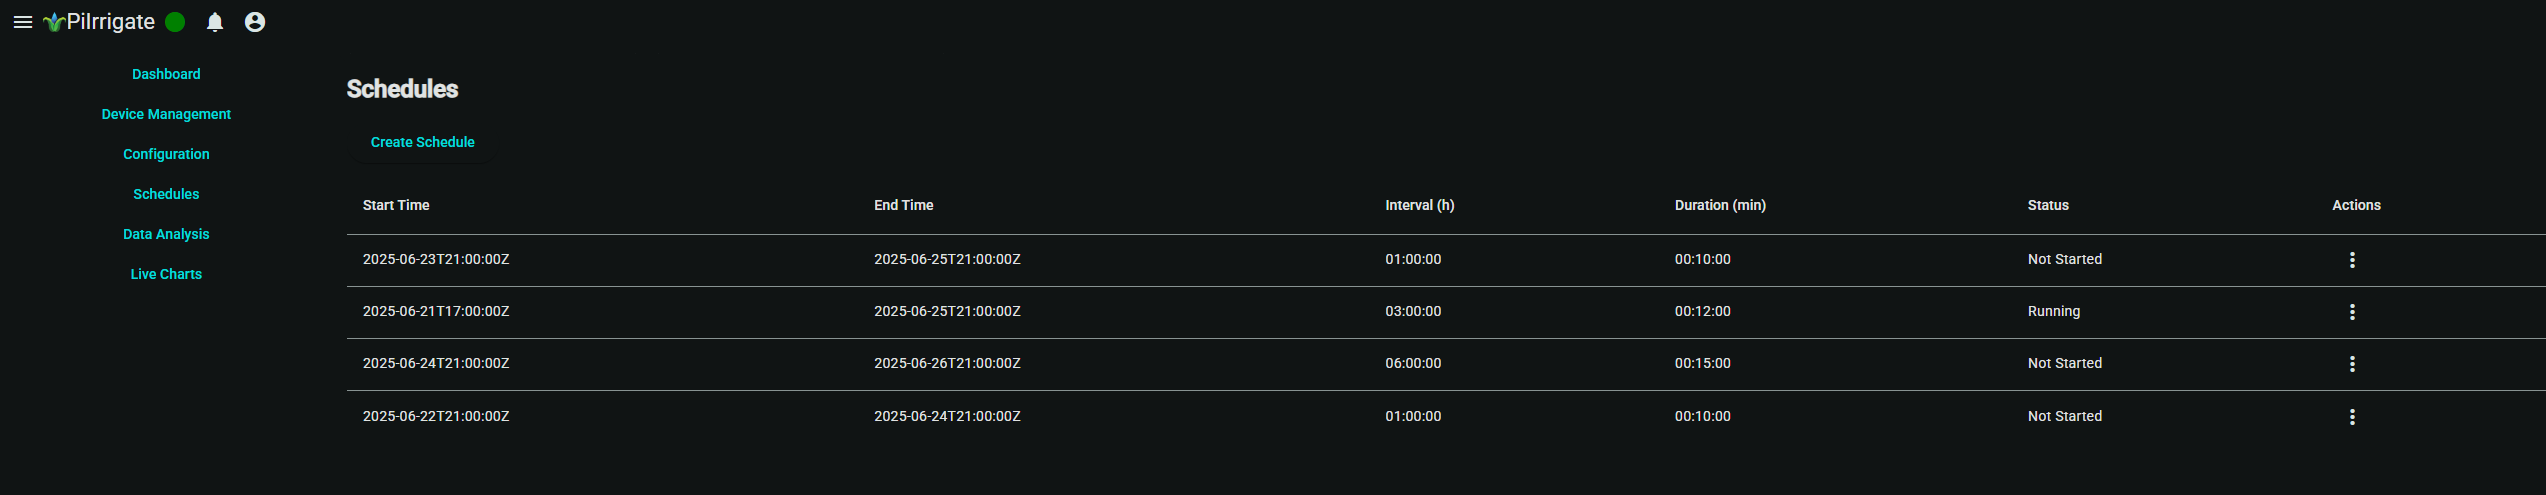
\includegraphics[width=0.8\textwidth]{images/schedules.png}
    \caption{Schedules page}
    \label{fig:schedules-page}
\end{figure}

\subsection{Data Analytics}
Data Analytics section allows the user to view the historical data collected from the sensors under the form of charts. One example 
of chart is shown in \ref{fig:analytics-page}. The user can also chose what features to display in the chart and it can also choose for what zone to
view the charts. 
\begin{figure}[H]
    \centering
    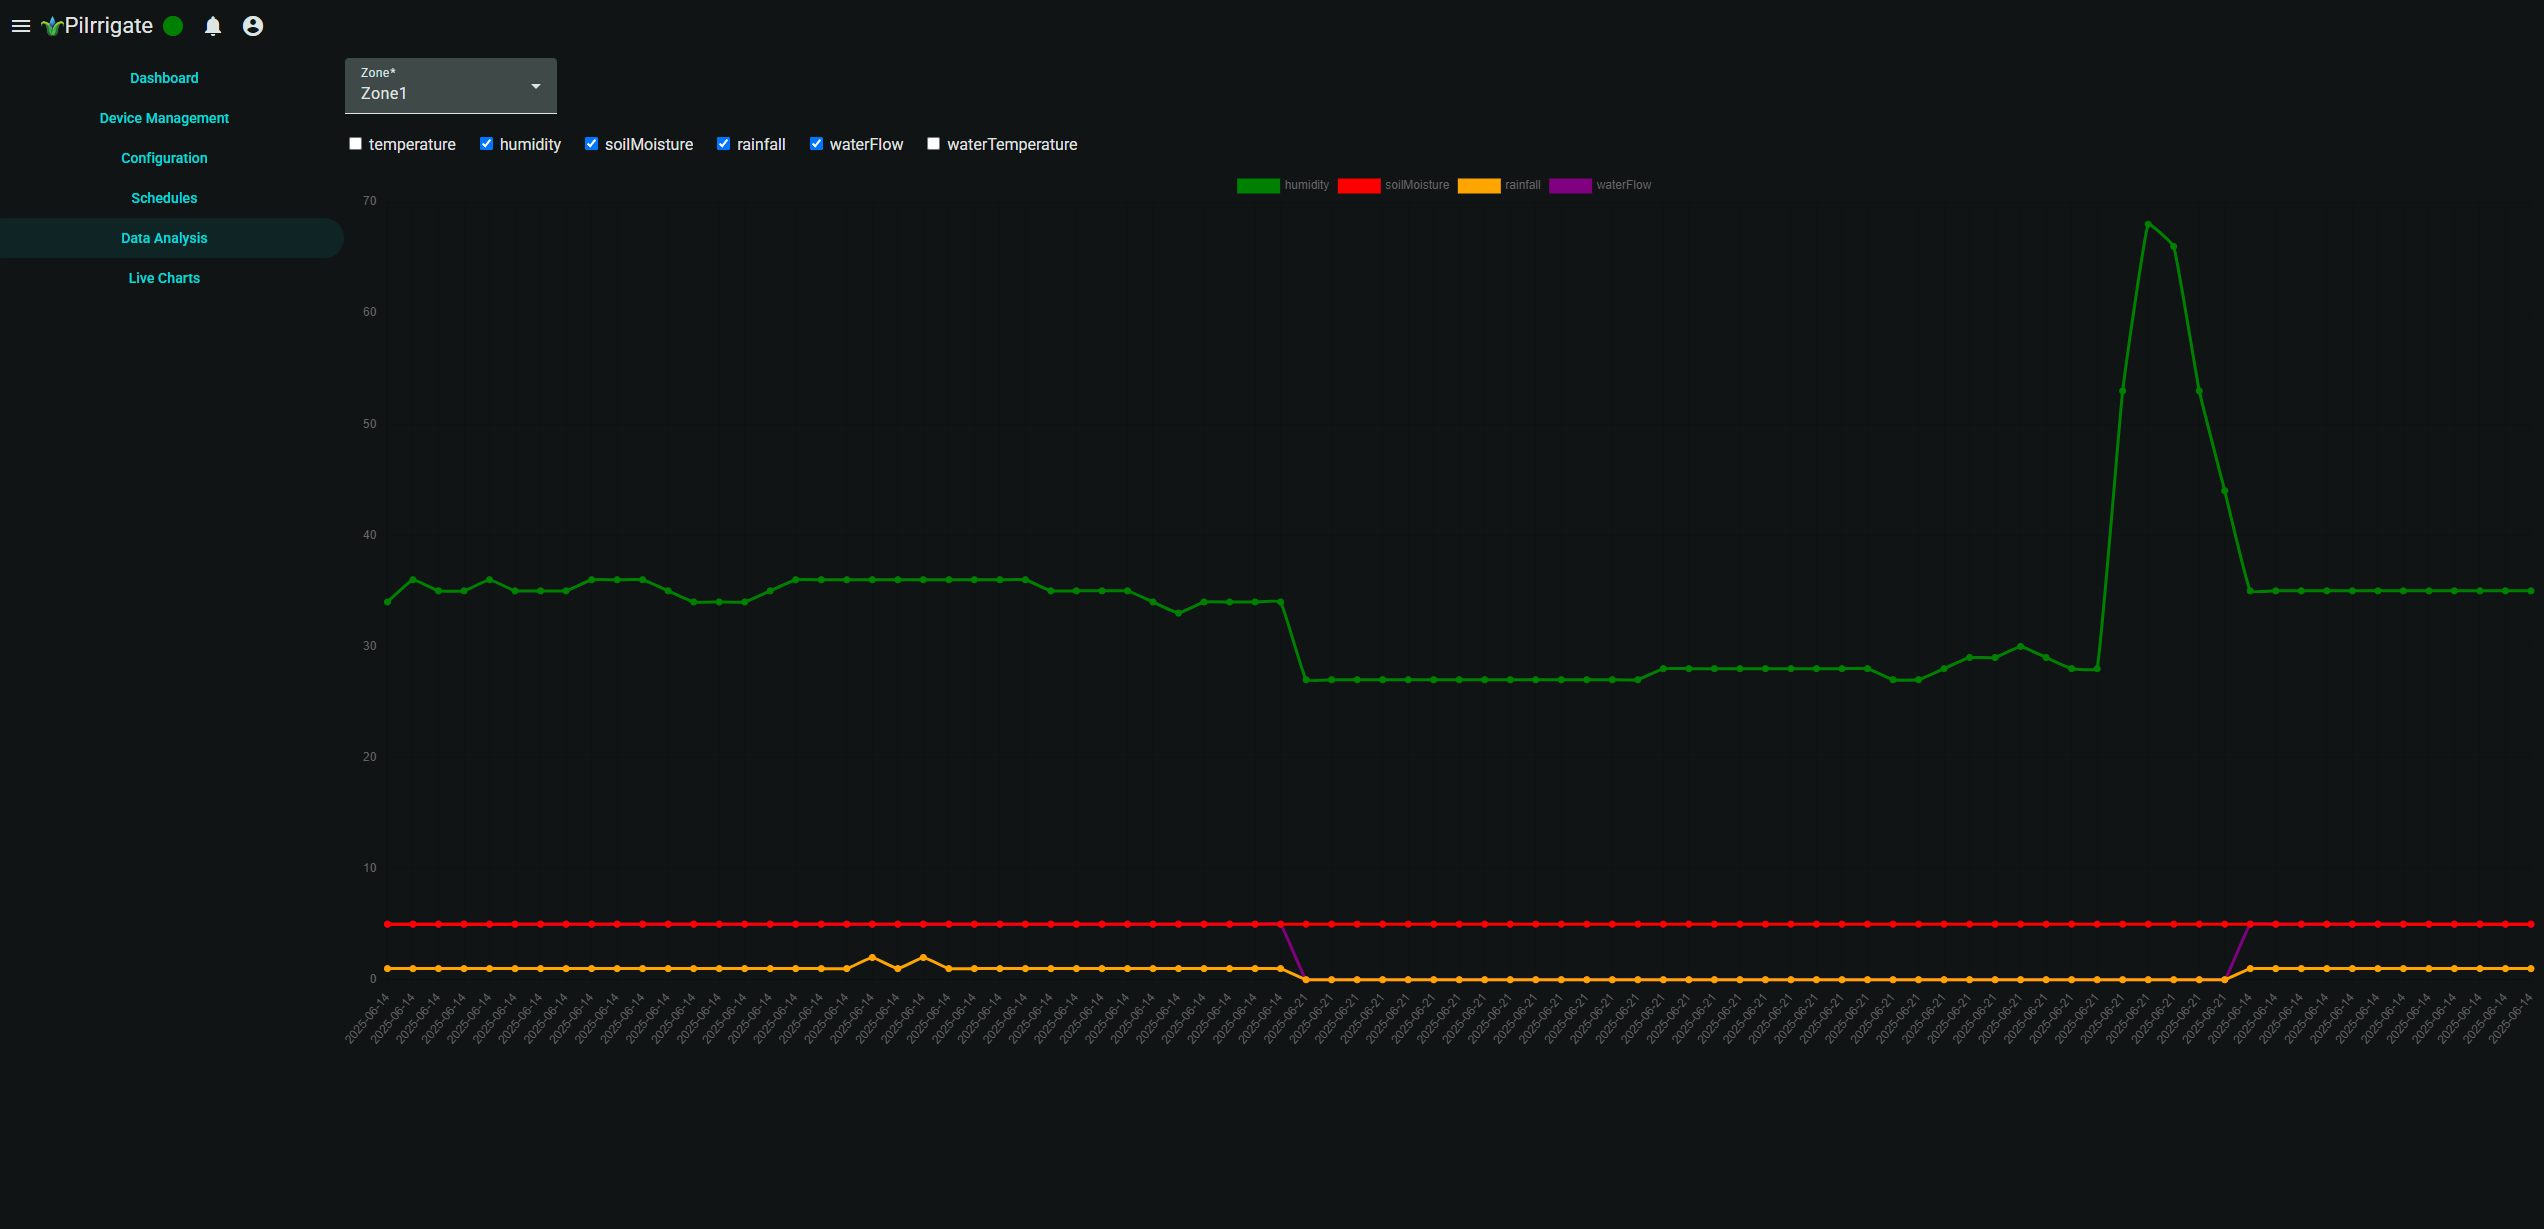
\includegraphics[width=0.8\textwidth]{images/analytics.png}
    \caption{Data Analytics page}
    \label{fig:analytics-page}
\end{figure}

\subsection{Live Charts}
In this section, the user can view in real time the data collected from the sensors, similar to the dashboard page. But in this case, the data is 
displayed in a chart format. The user can choose what features to display in the char and it can also choose for what zone to view the charts.
See \ref{fig:live-charts-page} for the Live Charts page.
\begin{figure}[H]
    \centering
    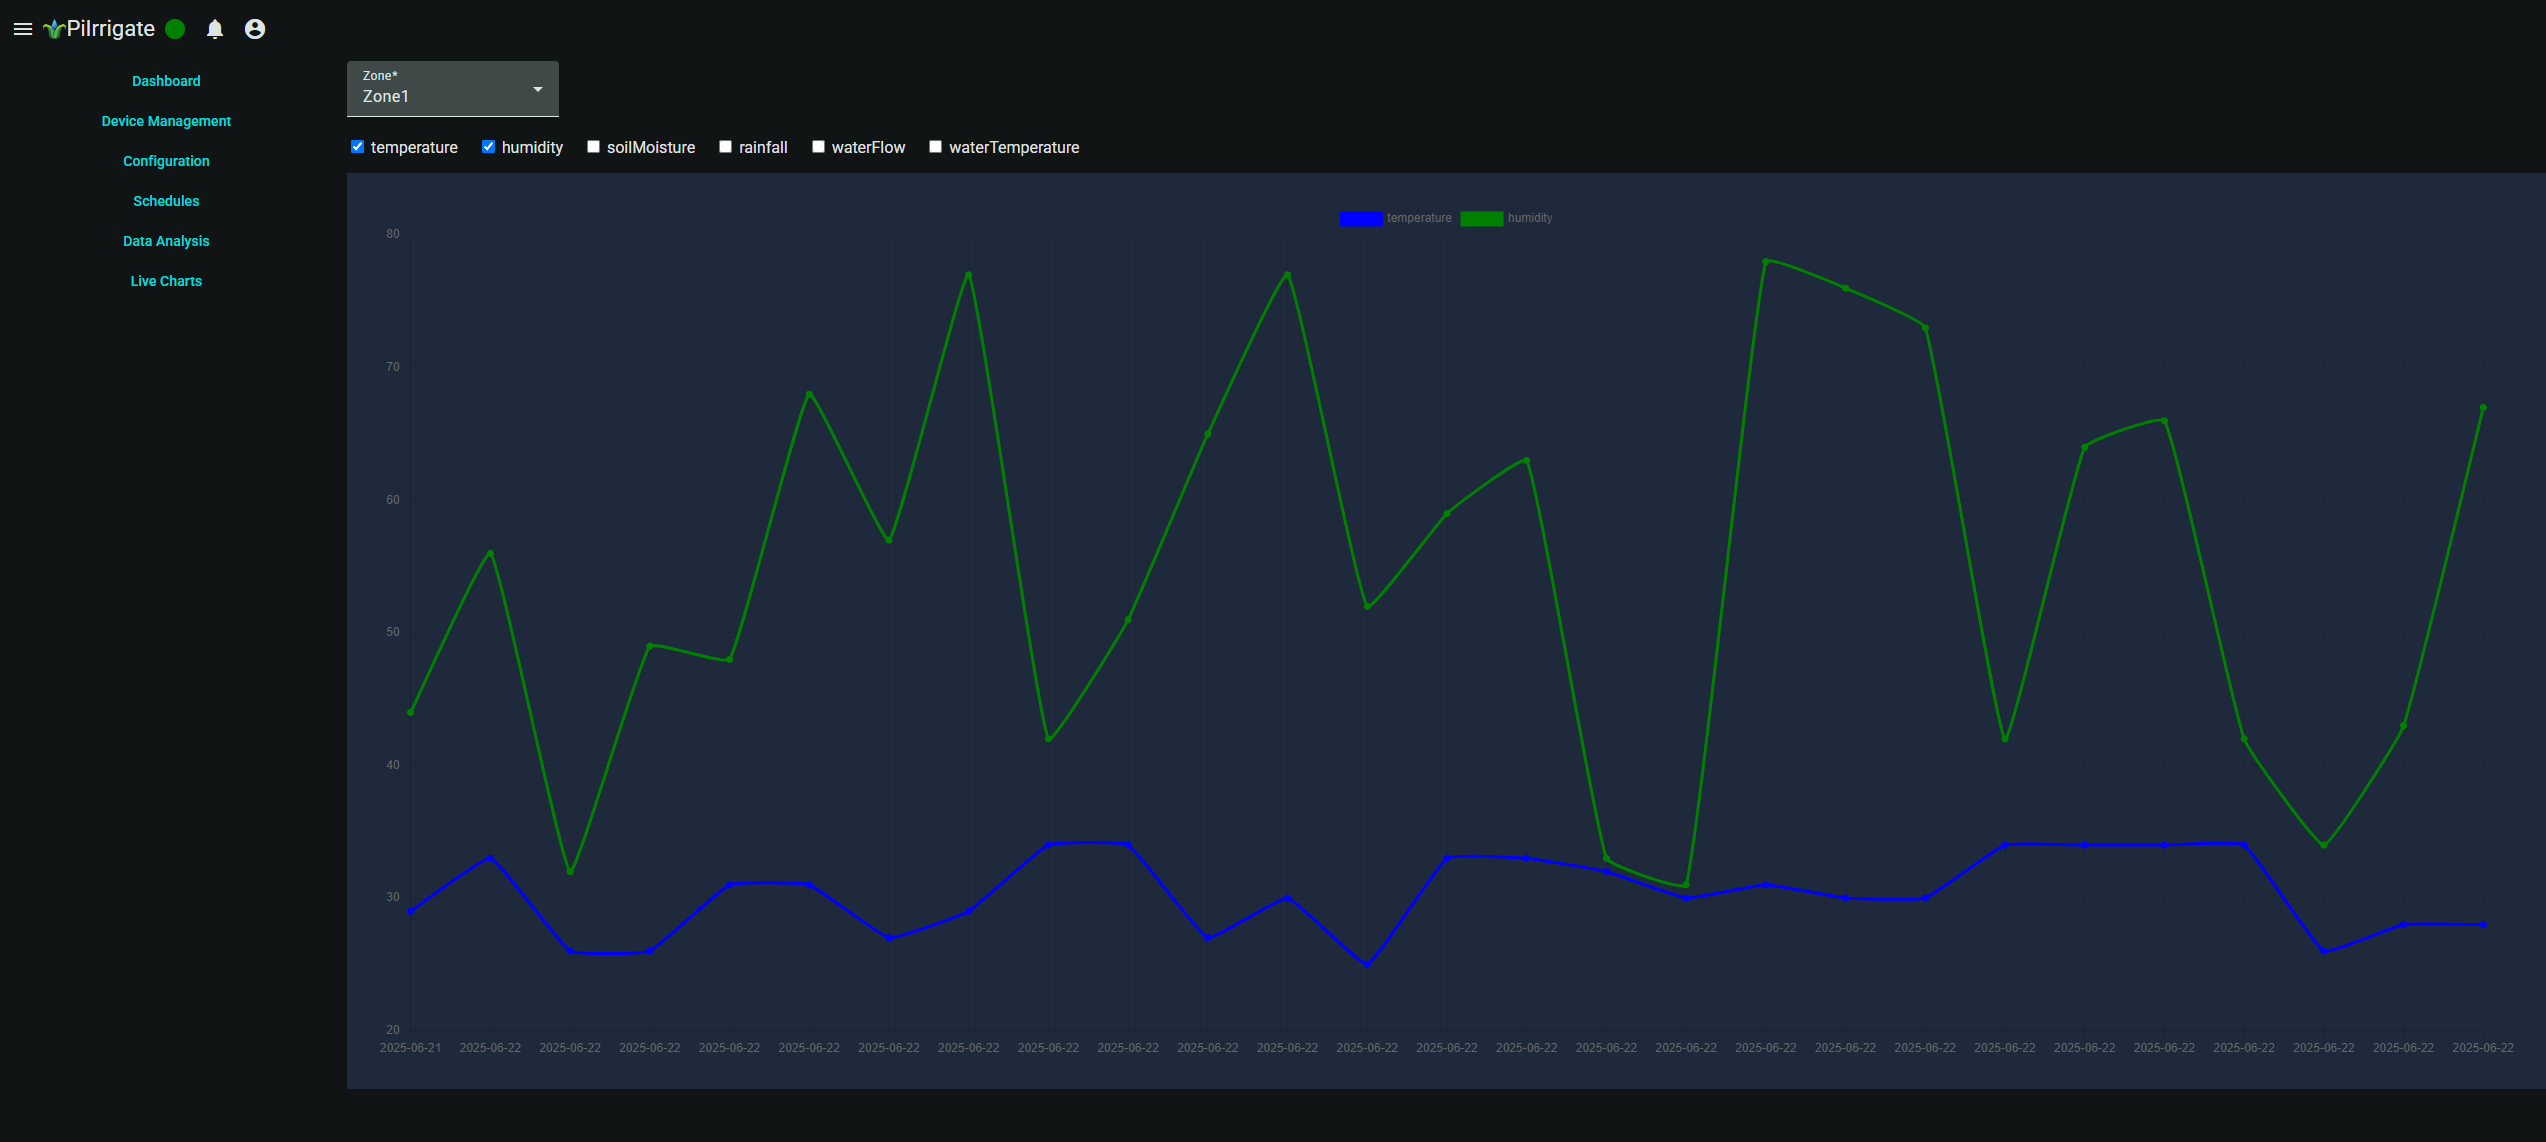
\includegraphics[width=0.8\textwidth]{images/live-charts.png}
    \caption{Live Charts page}
    \label{fig:live-charts-page}
\end{figure}


\section{Rule based system}
Automation is a key feature of the PiIrrigate system,
to achieve this, I implemented a rule-based system that allows the system
to make decisions based on the environmental data collected from the sensors.
The rule-based system is implemented in the Web API and it coonsists
of the following rules:
\begin{enumerate}
    \item If the soil moisture is below a certain threshold and the raindop sensor detects no rain, then start the irrigation.
    \item If the soil moisture is above a certain threshold and the water flow rate is above a certain level, the irrigation will be stoped.
    \item If the soil moisture reading is not available, then the irrigation will be stopped.
    \item If the soil moisture is below the threshold and the water flow rate is zero, then an alert will b sent to the user.
    \item If the irrigation process is running and the raindrop sensor detects rain, then stop the irrigation and send an alert to the user.
    \item If the water temperature is below or above a certain threshold, stop the irrigation, then send an alert to the user.
    \item If the water flow rate remains unchanged for a certain period of time, then send an alert to the user.
\end{enumerate}
This set of rules is executed every time a new sensor reading is received.
The rules are implemented in the IrrigaitonManager service which implements the IIrrigationManager interface.                                                   

\section{Used Technologies}
\subsection{Overview}
The PiIrrigate system is build using a variety of technologies, each serving a specific purpose. For programming
the ESP32, I used Arduino framework, within the Platform IO IDE. To handle the LoRa communication protocol I used \"LoRa.h\" library from developed by
Sandeep Mistry. The Raspberry Pi is programemd in Python
and it uses Azure IoT SDK for Python to communicate with the Azure IoT Hub. 
The web API it was developed in \.NET 8. The web application is developed in Anguler 19. The live communication between 
the web API and the web application is done using SignalR. The used database is PostgreSQL. The deployment of the web API and the web application
is done using Azure App Services.

\subsection{Programming Languges}
\subsubsection{C++}
C++ is a general-purpose programming languuage that is widely used in the embeded systems domain. It is well known
for its performance and efficiency. It supports multiple programming paradigms from procedural to object-oriented programming. 
The programing language was created in 1985 by Bjarne Stroustrup as an extension of the C programming language. On the top of C
, C++ adds features shuch as classes, inheritancem polymorphism, templates and exception handling.

\subsubsection {Arduino C++}
The firmware was developed using Arduino Framework. In this framework, the programing language used is a simplified version of C++.
The framework provides a set o libraries and APIs that are meant to abtract the low-level details of the hardware operations. Some of the
mose used functions are digitalRead, digitalWrite, analogRead, delay, etc.

\subsubsection{Python}
Python is a high-level, interpreted programming language. The language was created By Guido van Rossum and it was first released in 1991.
It is well known for it's reability, simplicity and versatillity. Python supports multiple programming paradigms, like functiona, procedural and
object-oriented programming. It can be used for a wide range of applications, from web development to data science and machine learning.
In the PiIrrigate system, Python was used to develop the Raspberry Pi gateway. 

\subsubsection{C-Sharp}
C\# is a modern object oriented programming language developed by Microsoft. It was first released in 2000 as part of the \.NET framework.
It was designed to be simple robust and versatile. C\# combined the performance of compiled languages with the ease of development offers
typical of managed languages. It supports modern programming features such as generics and it is a strongly typed language\cite{dotnet_official}\cite{microsoft_csharp}.
In the PiIrrigate system, C\# was used to develop the web API.

\subsubsection{TypeScript}
TypeScript is a statically typed language. It is a superset of JavaScript and was designed to enchance the scalability and maintability of large codesbes.
It introduced intefaces, decorators, enums and generics while maintaining compatibility with existing JavaScript code. Typescrip became
the standard for developing large applications, especially when using frameworks like Angular. Typescrips was used to develop the Angular
web application in the PiIrrigateSystem. It was chosen because it provides a better development exceperience.

\subsection{Frameworks and SDKs}
\subsubsection{Ardunio Framework}
Arduino framework is an open-source electronics development platform that enables developers to create project on a wide rande of microcontrollers.
It provides a wide range of libraries (ex: LoRa.h, Wifi.h, HTTPClient.h, etc). The integration is very smooth with both Arduino IDEa and Platform ID.
I used the Arduino framwerk to develop the ESP32 firmware because it's ideal for rapid prototyping and it is widely use in this kind of projects\cite{arduino_core}.

\subsubsection{Azure IoT SDK for Python}
Azure IoT SDK for Python consist of a set of libraries that allows developers to interact with Azure IoT Hub. I chose the client
library to connect the Raspberry Pi the Azure IoT Hub. More specifically I used the telemetry transimission feature to send the sendor readings 
to the cloud. The SDK offers suport for multiple protocols, including MQTT, AMQP and HTTP\cite{azure_iot_hub_docs}\cite{azure_iot_sdk_python}.

\subsubsection{dotNET 8}
\.NET 8 is the latest version of the \.NET framework, a cross-platform, open-source framework for building applications. It is supported by Microsoft
and it is widely used to build web application, web APIs, desktop applicaitons and even mobile applications. It offers support for multiple programming
languages, including C\#, F\# and Visual Basic. \.NET 8 was used to implement a RESTful backend API for the PiIrrigate system, 
which prvides the neccesarry endpoints for user management, data storage, and communication with the IoT Hub. Another important aspect of \.NET 8
is that it has natice support for asynchronous programming, dependency injection\cite{dotnet8_docs}\cite{microsoft_dotnet}.

\subsubsection{Entity Framework Core}
EF Core is an open-source ORM\. It is developed by Microsoft and it is part of the \.NET framwork. It enables developers
to work with databases using class objects. Most of the raw queries that are usualy used in SQL databases are replaced with LINQ queries, 
wich are more readable and easier to maintain. EF core supports multiple database, including SQL Server, PostgreSQL, MySQL and SQLite.
It was used in this project to interact with the PostgreSQL database\cite{efcore}\cite{efcore_docs}.


\subsubsection{Angular 19}
Angular is an open-source frontedn web application framework maintained by Google. It can be used to build SPAs. The framework is written in 
TypeScript and it provides a set of tools and libraries for building modern web applicaitons. Angular is based on components, which are reusable. 
With the last version, Angular shifts to a more modular architecture, more and more components are being developed as standalone components.
Angular 19 was used to develop the web application for the PiIrrigate system\cite{angular_19_release}\cite{angular_docs}.

\subsection{Component Libraries}
\subsubsection{Angular Material}
Angular Material is a UI compoent library thath implements the Material Design specification.
It was created by the Angular team at Google and it provides a wide range of reusable compoenents, including 
buttons, crdsm tables, dialogs, and form controls. By using Angular Material in the UI development, the apps obtained are consistent
and visually appealing, while also being responsive and accessible. Another aspect of using component libraries is thah 
it reduces the amount of custom CSS that needs to be written, as most of the components come with prebuild style and themes\cite{material_design_spec}\cite{angular_material_docs}.


\subsection{Libraries}
\subsection{LoRa.h}
Lora.h is a libray developed by Sandeep Mistry that provides an easy way to use LoRa communication protocol. 
It is intednded for Semtech Semtech SX1276/77/78/79 based boards/shields\cite{arduino_lora_lib}.
In this project I used the following functions from the libray: 
\begin{enumerate}
    \item begin() - to initialize the LoRa module.
    \item beginPacket() - to start a new LoRa packet.
    \item endPacket() - to send the LoRa packet.
    \item parsePacket() - to check if a new LoRa packet is available.
    \item readbytes() - to read the data from the LoRa packet.
    \item readStringUntil() - to read a string from the LoRa packet.
\end{enumerate}

\subsubsection{SignalR}
SignalR is a libray built by Microsoft as part of the \.NET framework. It provides real-time web functionality to applications, allowing bidirectional
communication between the server and the client. It is used to send real-time updates to the web application form the web API 
without the need for the client to poll the server\cite{signalr_docs}.

\subsection{Cloud and Hosting}
\subsubsection{Azure App Services}
Azure App Service is a fully managed PaaS that allows developers to deploy web appicaitons, RESTful APIs without having to manage the
underlying infrastructure. It supports multiple programming languages, including \.NET, Python, Node.js, and Java. It can be
easly integrated with CI/CD pipelines and it provides build-in support for scaling, monitoring and security\cite{azure_app_service}.
In the PiIrrigate system the deploy was done using the Publish feature of Visual Studio. With a few clicks, the web API and the web applicaiton
were deployed to Azure AppServices.

\subsubsection{Neon Database}
Neon is a fully managed serverless PostgreSQL database platform. It is designated for moder cloud-native applications. It is 
designed to be easy to use, scalable and cost-effective. Neon provides a serverless architecture and it separates the storage and the compute layers,
allowing for automatic scaling and high availability.

\subsection{Development Tools}
\subsubsection{Platform IO}
Platform IO is an open-source IDE that comes as a VSCode extension. It supports a wide range of platforms, including the ESP32.
They have an unique philosophy in the embeded market, which is to provide developers withs a modern integrated development environment that
allows them to access a wide range of libraries and frameworks. Besides that, Platform IO works cross-platform and offers uni testing, automatic code
analysis and debbuging capabilities\cite{python_org}\cite{python}\cite{peps}.

\subsubsection{Visual Studio Code}
Visual Studion Code is a free open-source code editor. It is developed by Microsoft and it is available on all major platforms.
The editor is higly customizable and it supports a wider range of programming languages. In this project, I used VSCode 
as the main IDE for developing the ESP32 firmware, the web appication and also the code for the Raspberry Pi was written using VSCode. One of the nice
fetures of VSCode is that supports SSH connections, which alllowed me to edit and run the code on the Raspberry Pi directly from the integrated terminal
\cite{visualstudio_docs}.

\subsection{Visual Studio}
Visual Studio is an IDE developed by Microsoft. It is available only on Windows and it is used to develop applications with the \.NET framework.
The IDE provides a wide range of tools for debugging, profiling, testing and deploying applications. 
In this project, I used Visual Studio to develop the web API\cite{github_docs}.

\subsection{Github}
Github is a web-based platform for version control and collaboration. It is built on the top of Git and it allows developers to host and manage 
code repositories, track changes and collaborate with other developers. It supports continuous integration and continous deployment pipelines,
which automates the build, test and deployment processes\cite{github_docs}. In this project, I used Github to host the code repositories for the entire system.

\subsection{Draw.io}
Draw.io is a free online diagramming tool that allows users to create flowcharts, UML diagrams and other types of diagrams.
It was used to create all the presented diagrams.